\documentclass[UTF8]{ctexart}
\usepackage{shumo}%可以点开查看宏包和定义内容，同时可以自行另外加宏包和定义
\usepackage{hyperref}
\hypersetup{colorlinks=true,linkcolor=black,citecolor=black,urlcolor=black}
\geometry{left=2.5cm,right=2.5cm,top=2.5cm,bottom=2.5cm}%页面布局集训标准，可自行适当修改
%====================================================
%设置附录代码的格式，可以自行修改
\lstset{
	breaklines=true,% 允许自动断行
	% breakatwhitespace=true,% 使用此命令仅允许在空格处自动断行
	showstringspaces=false,% 不显示字符串中的空格
	basicstyle=\small\ttfamily,% 设置代码基本样式
	flexiblecolumns=true,% 改善字母间距
	keywordstyle=\color{blue},% 设置关键词样式
	stringstyle=\color[rgb]{0.75,0,0.75},% 设置字符串样式
	commentstyle=\songti\color[rgb]{0,0.5,0},% 设置注释样式
	tabsize=4,% 设置制表符缩进
}
%====================================================
\title{\textbf{基于红外干涉法的SiC外延层厚度测算}}% 请勿修改
\date{}%请勿添加自己的信息
\author{}%请勿添加自己的信息
%下面时正文
\begin{document}
\setcounter{page}{1}%从正文开始计算页码	
\maketitle
\vspace{-0.95cm}
\thispagestyle{fancy}   
%\fancyhf{} %清除原本页眉页脚形式
\renewcommand{\headrulewidth}{0pt} %页眉线宽，设为0可以去页眉线
%=================================================
%=================================================
%=================================================
%=================================================
%=================================================
%=================================================
%下面开始出现各位需要修改的部分。
\renewcommand{\abstractname}{\sihao 摘\quad 要} %更改摘要二字的样式
\begin{abstract}\xiaosihao
	\vspace{0.1cm}
 SiC 是第三代半导体材料的代表，对 SiC 的利用基于其外延层，外延层厚度的测算对材料效能有重要影响。本文基于红外干涉法，分别建立并求解双光束以及多光束干涉下外延层厚度计算模型，解决了单次反、透射和多次反、透射的外延层厚度求解问题；并分析了多光束干涉产生条件与影响。\par 
 \textbf{针对问题一，}聚焦波长与载流子浓度建立\textbf{折射率计算模型}，分析干涉现象建立\textbf{干涉极值级数计算模型}，搭建基于折射率和干涉极值级数的\textbf{外延层厚度计算模型}。综合考虑晶格振动，载流子浓度与红外光谱的波长
 ，基于光波的角速度经验公式，并对自由载流子浓度取合理常值，建立仅与波长相关的折射率计算模型；干涉极值对应反射率曲线的波谷，建立干涉极值级数关于波数的表达式；结合SiC外延层厚度计算公式，将干涉极值级数的表达式，以及折射率计算模型，代入得到关于波数、折射率以及入射角的SiC外延层厚度计算模型。\par 
 \textbf{针对问题二，}通过\textbf{波谷分析}，求解稳定的干涉极值级数，对应计算相应波数时的折射率，代回SiC外延层厚度计算模型，对求解结果取均值，得到最终的外延层厚度模型求解结果。首先对附件1，2数据进行数据分析以及降噪处理；将附件波数数据转换为波长代入折射率计算模型，分别求解入射角为$10^\circ$与$15^\circ$时，各波数对应的折射率；通过波谷分析对波谷（干涉极值）的取值进行筛选，根据\textbf{波谷分布特征}，选取干涉现象稳定的波谷，根据选取的波谷数据，确定对应的波数，并求解相应的折射率数据结果；将选定的波数与折射率数据代入SiC外延层厚度计算模型，求解得到选取的外延层厚度计算结果，对该结果求均值，得到最终的SiC外延层厚度结果：16.6$\mu m$（附件1），17.6$\mu m$（附件2）。\par 
 \textbf{针对问题三，}在对\textbf{多光束干涉必要条件及影响分析}的基础上，判断多光束干涉是否在附件数据中存在，建立并求解相应的\textbf{多光束干涉下外延层厚度计算模型}。首先，理论分析干涉及多光束干涉明显的必要条件，综合得到多光束干涉必要条件；分析多光束干涉对相位分布产生影响，进而影响外延层厚度信息识别（计算精度）；附件数据均出现多光束干涉；\textbf{硅晶圆片外延层厚度计算}上，先基于\textbf{色散经验公式}建立折射率求解模型，而后基于多光束干涉的分析，将总反射率计算公式转化为，总反射率，位相差与外延层表面反射率相关的反射率函数，通过位相差关于外延层厚度的表达式建立反射率函数与厚度的关系，综合得到Si的多光束干涉下外延层厚度计算模型；通过\textbf{最小二乘法}拟合反射率函数中的外延片厚度参数$D$，使其与附件数据实际反射率的残差平方和最小，\textbf{附件3，4厚度求解结果分别为:4.7577$\mu m$}和$4。5593\mu m$(MSE:0.9759353)；\textbf{碳化硅晶圆片外延层厚度的计算}上，根据多光束干涉下总反射率推导过程，推导双光束干涉的总反射率函数，并对多光束干涉下的总反射率函数进行变形，比较得到多光束干涉时增加了一项补偿项$\frac{1}{1-Re^{i\sigma}}$；为减少多光束干涉影响，则尽量使$Re^{i\sigma}$趋于0，即反射率$R$应尽可能小，求解得到附件1，2外延层厚度分别为：16.2416$\mu m$和17.4144$\mu m$。\par 
 \textbf{关键词}:\quad 碳化硅外延层厚度\ 菲涅尔公式\ 波谷分析\ 色散经验公式\  
\end{abstract}
\newpage
\pagestyle{plain}
%标准 LaTeX 提供下列四种页版式，可用 \pagestyle{页版式} 命令来设置页面版式：
%empty(没有页眉和页脚)，plain(本次用的，无页眉，页脚为居中页码)，headings(页眉为章节标题，无页脚)，myheadings(页眉内容可自定义，无页脚)


\section{问题重述}
\subsection{问题背景}
第三代半导体材料在各方面较前两代优势明显，其中的典型代表碳化硅（SiC）由于其物理化学特性非常优异，备受瞩目。在使用SiC材料制造器件时，直接使用其单晶材料有许多弊端，且成本高昂，在制造工艺上通常采用外延技术。外延技术使SiC材料的单晶衬底上生长出外延层，基于外延层进行器材加工。所以在半导体的加工上，外延层的厚度对于半导体器件的使用性能有重要影响。\par 
基于外延层厚度的重要影响，外延层厚度的测算十分必要。在高精度仪器厚度测量上，对器件不会造成损伤的方法主要有红外干涉法等。红外干涉法是通过红外光线照射SiC，光线分别在外延层与衬底发生反射，两条反射光线在某种条件下产生干涉，根据干涉条纹与波长、折射率以及外延层厚度之间的关系，可以通过干涉条纹分析SiC的外延层厚度。红外干涉法测算外延层厚度的示意图如下：\par 
	\begin{figure}[H]
	\hspace{1cm}
	\begin{minipage}{0.3\textwidth}
		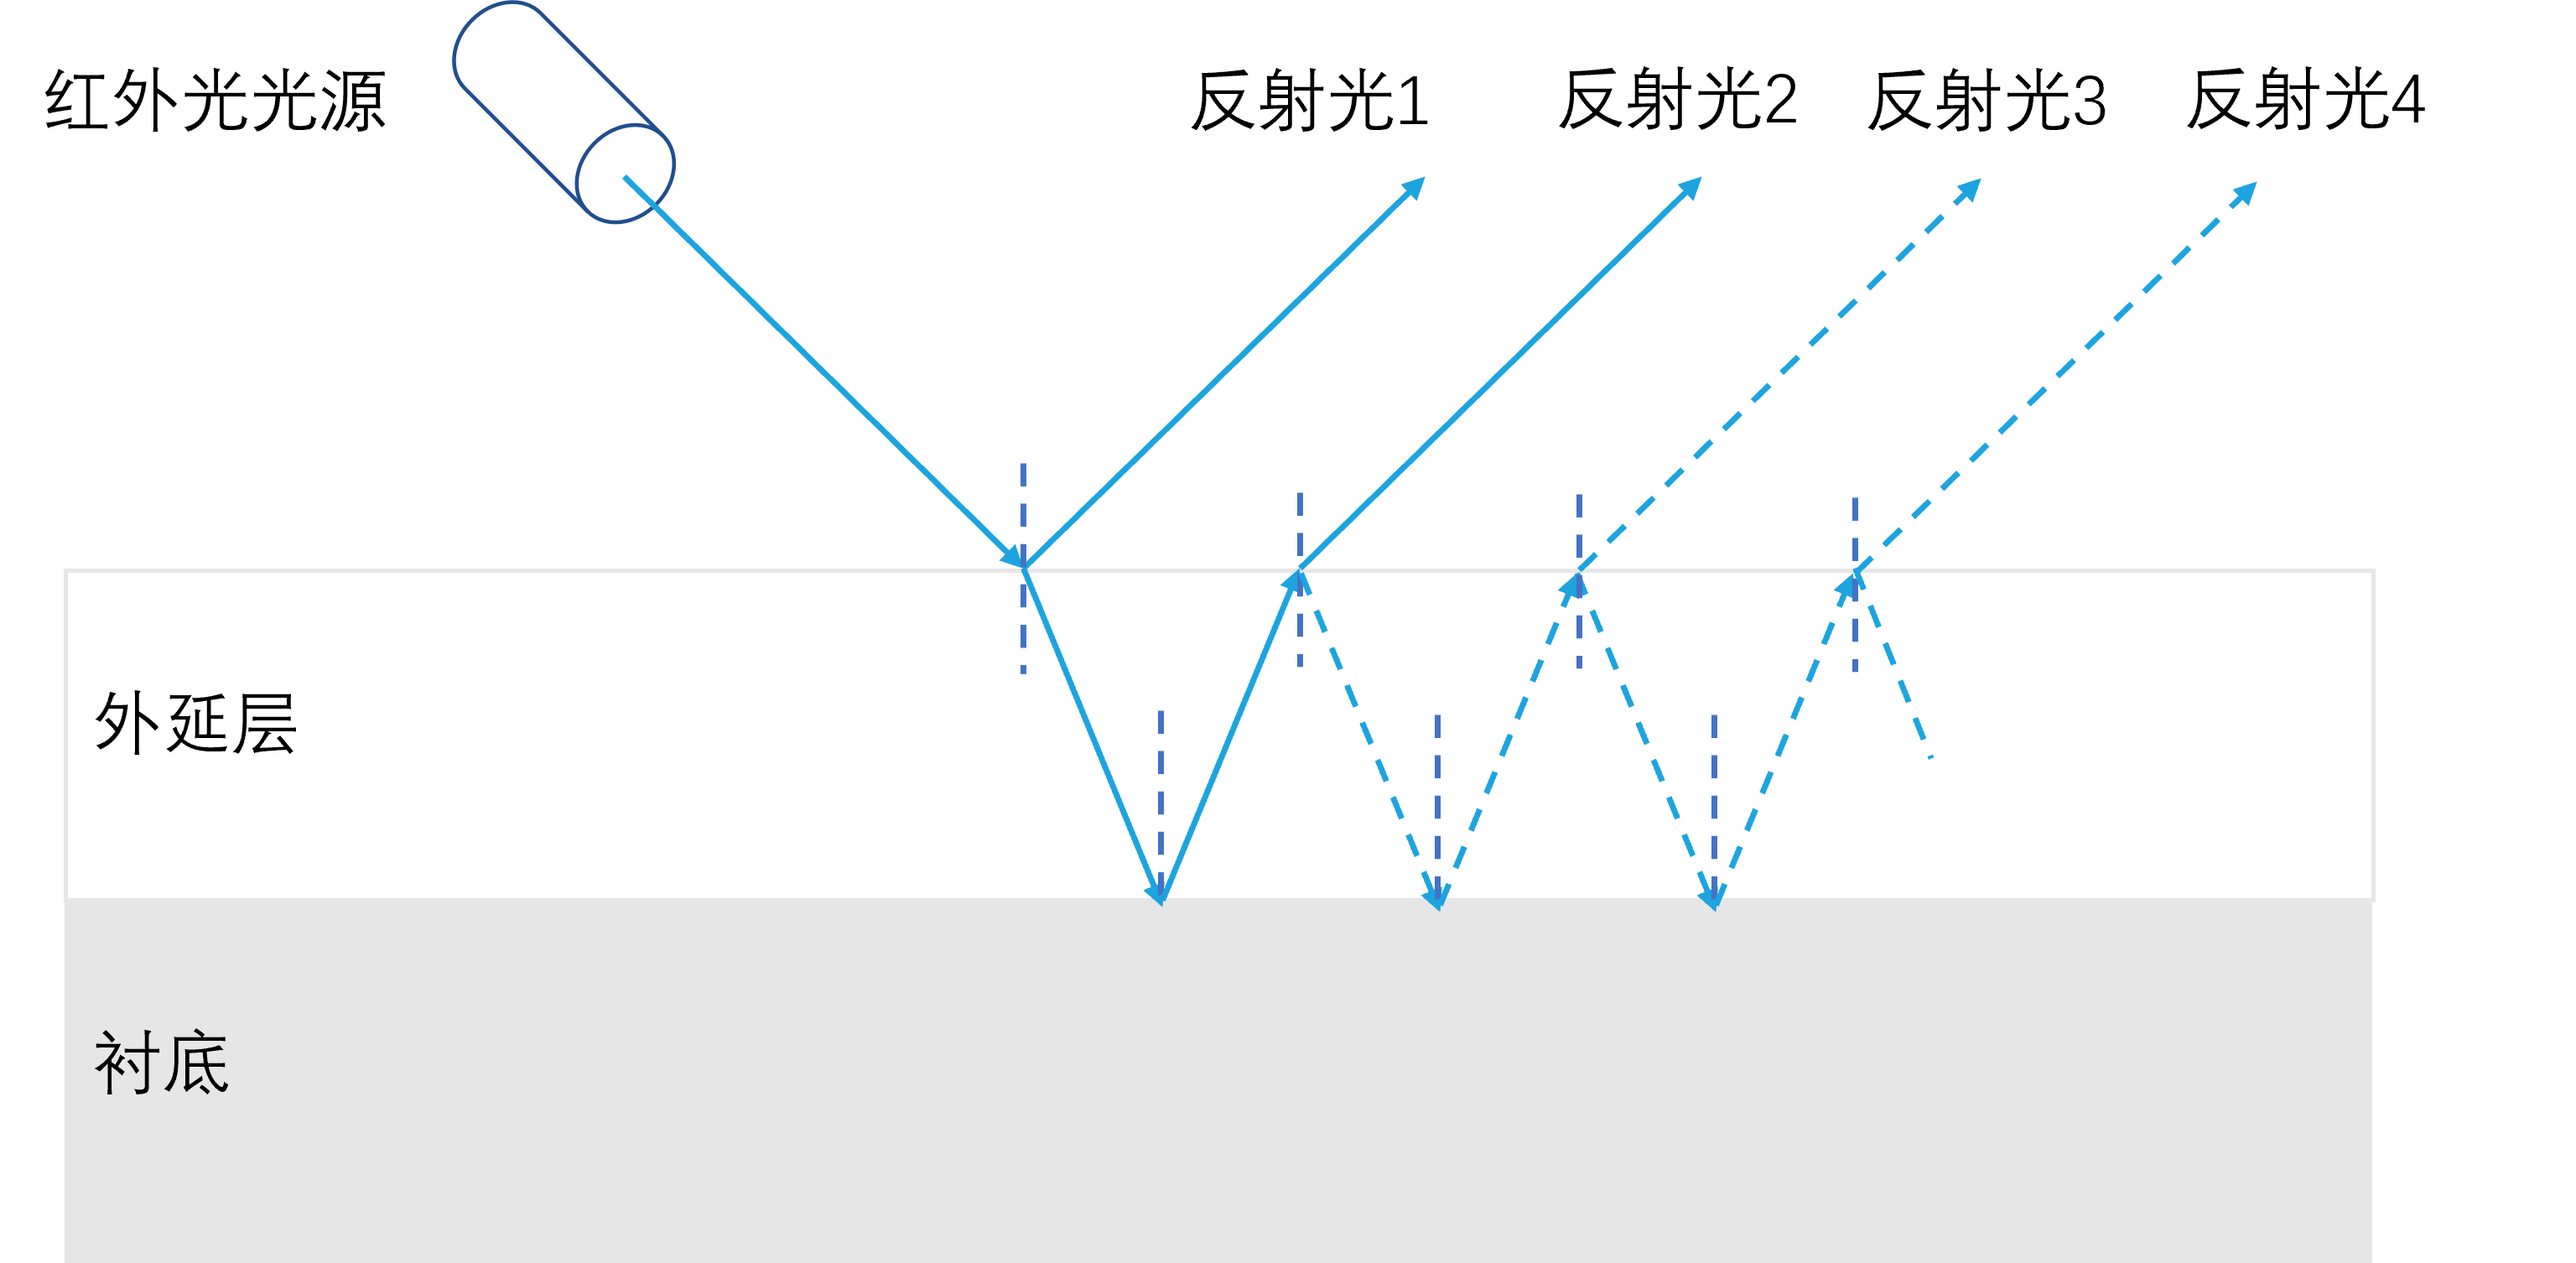
\includegraphics[height=0.3\textheight]{p1.png}
	\end{minipage}  
	\caption{红外干涉法测算SiC外延层厚度示意图}
\end{figure}\par   
\subsection{问题提出}
针对SiC外延层厚度测算需求，逐步深入地建立数学模型对SiC外延层的厚度进行测算：\par 
1.简化红外干涉法测算SiC外延层厚度的模型，，将光波的反射与透射简化，仅考虑单次反射与透射的情形，建立合适的数学模型，在波长、入射角、折射率以及外延层厚度间建立起联系，得到可对外延层厚度求解的模型。\par 
2.在得到外延层厚度求解模型的基础上，进行算法设计，利用合适的求解算法，对提供的附件材料进行外延层厚度求解。附件提供两组SiC的光谱实际测量数据，分别对应$10^\circ$以及$15^\circ$入射角的测试情景。在求解得到两组SiC对应的外延层厚度结果的基础上，对结果进行分析，说明结果是可靠的。\par 
3.在实际情境中，光波的反射与投射并不是单次的，为了实际测算需求，必须对模型进行推广，将光波的反射与透射考虑为多次。多次的反射与透射会带来多束光的干涉，影响外延层厚度测算的精度。为避免多数光的干涉，需要对多束光干涉产生的条件进行分析，找到产生的必要条件，以及干涉的产生对外延层厚度测算精度的影响，并根据该条件的标准，判断附件关于硅晶圆片的实测数据，有无多光束的干涉，并建立在多束光干涉下的硅晶圆片外延层厚度测算模型，并根据算法求解外延层厚度。进一步地对SiC的圆片进行判断，是否存在多束光干涉，若存在寻找方法消除多光束干涉影响，并求解消除影响后的厚度计算结果。\par 
\section{问题分析}
\subsection{问题一分析}
根据题目要求，建立数学模型实现外延层厚度的计算，先查询红外干涉法计算外延层厚度的原理，并寻找对应的计算公式。根据红外干涉法的原理，外延层厚度的求解与干涉现象产生的干涉条纹极值级数、入射角、折射率、波长等相关。进一步地对干涉条纹极值级数、折射率、波长的信息进行分析，结合题目已知数据：入射角、波数与反射率，需要找到已知数据与公式变量间的联系。先对折射率的计算进行分析，考虑到问题二中需要对模型进行求解，所以基于已知数据建立测算模型，根据题目已知数据：反射率，寻找相关联的折射率计算公式。进一步对干涉振幅，进行分析，找到对应的计算表达式。完成模型准备后，根据已有的外延层厚度计算表达式，进行模型搭建。\par 
\subsection{问题二分析}
本题为问题一的延伸，是对问题一的模型进行求解分析，对问题一建立的模型进行实测数据验证模型的可解性，并且对实测数据进行求解分析，检验问题一所建模型的的可靠性。在问题一建立的模型的基础上，对模型进行求解。在问题一中分析得到需要进行求解的数据有：干涉级数、折射率。干涉级数可通过对干涉现象在反射率与波数曲线上的分析得到。折射率的求解计算，考虑两种方案，若问题一中建立的折射率函数可解，则对函数求解，得到解析解结果；若函数不可解，则考虑通过对折射率函数进行分析，寻找反射率数据对应的数值解。求解得到上述数据后，通过厚度计算公式，进行外延层厚度求解，求解得到的结果应符合标准范围，且符合实际情况，根据标准进行分析，分析求解结果是否可靠。\par 
\subsection{问题三分析}
本题是对问题一二的拓展，考虑光线在外延层与衬底间发生多次反射与透射，多次反射形成多条反射光线，多条反射光线在外延层外发生干涉现象，形成多光束干涉的情况。但是多光束干涉的产生并不是一定的，所以先需要对产生该情况的条件进行分析，推理得到相关的必要性条件，并分析产生多光束干涉现象相较于双光束干涉现象，对使用红外干涉法测算外延层厚度在精度上会产生什么影响。\par 
在整体理论分析多光束干涉影响的基础上，逐层深入地探究多光束干涉在实际测算外延层厚度时，会产生什么影响。\par 
(1)先对硅晶圆片进行讨论，根据整体的理论性分析结果，依据多光束干涉的形成条件，分析通过红外干涉法进行硅晶圆片外延层厚度的测算时，是否存在多光束干涉现象；并基于分析结果，对硅晶圆片的外延层厚度进行模型设计，建立合适的模型描述外延层厚度与已有实测数据之间的关系，并且通过一定的算法对其外延层厚度进行求解。\par 
(2)进一步地对碳化硅晶圆片进行分析，判断在问题一二进行求解外延层厚度的实测数据背景中，干涉现象是否为多光束的干涉现象，根据判断结果选择，对原碳化硅外延层厚度求解的模型进行修正，通过修正消除，多光束干涉对SiC外延层厚度求解精度的影响，并使用合适方法求解外延层厚度。\par 
\newpage 
\section{符号说明}
\begin{table}[H]
	\centering
	\begin{tabular}{ccc}
		\toprule[1.5pt]
		\makebox[0.3\textwidth][c]{变量名}&\makebox[0.4\textwidth][c]{符号说明}&\makebox[0.2\textwidth][c]{单位}\\
		\midrule[1pt]
		$R_S$&垂直偏振平面的反射率&\\
		\addlinespace
		$R_p$&平行偏振平面的反射率&\\
		\addlinespace
		$r_S$&垂直偏振平面的振幅系数&\\
		\addlinespace
		$r_p$&平行偏振平面的振幅系数&\\
		\addlinespace
		$R$&非偏振光的反射率&\\
		\addlinespace
		$T$&非偏振光的透射率&\\
		\addlinespace
		$R_t$&总反射率&\\
		\addlinespace
		$I$&光强&\\
		\addlinespace
		$\lambda$&红外光波长&\\
		\addlinespace
		$k_i$&第i个极值对应的波数&\\
		\addlinespace
		$P_i$&第i个极值对应的级数&\\
		\addlinespace
		$D$&外延层厚度&\\
		\addlinespace
		$\theta_i$&入射角&$\circ$\\
		\addlinespace
		$\theta_t$&折射角&$\circ$\\
		\addlinespace
		$P$&载流子浓度&\\
		\addlinespace
		$m^*$&有效电子/空穴质量&\\
		\addlinespace
		$c$&光速&\\
		\addlinespace
		$n_i$&环境折射率&\\
		\addlinespace
		$n_t$&外延面折射率&\\
		\addlinespace
		$\lambda_i$&第i个极值处的波长&\\
		\addlinespace
		$m$&极数差&\\
		\addlinespace
		$k$&对比度&\\
		\addlinespace
		$k$&对比度&\\
		\addlinespace
		$\phi_g$&光程差对应的相位差&\\
		\addlinespace
		$\phi_f$&界面反射相移对应的相位差&\\
		\addlinespace
		$\phi$&反射光相位差&\\
		\addlinespace
		$\omega$&光波的角频率&\\
		\addlinespace
		$\delta_0$&位相差常数&\\
		\addlinespace
		$\delta$&位相差&\\
		\bottomrule[1pt]
	\end{tabular}
\end{table}
\section{模型假设}
1.假设衬底不会对红外光有吸收\par
2.假设环境由纯氮气填充\par
\newpage
\section{模型的建立与求解}
\subsection{问题一：外延层厚度计算模型建立}
\subsubsection{模型准备}
为避免环境中水蒸气或二氧化碳对红外光的吸收，测算外延层时，环境通常采用纯氮气填充，根据相关文献，氮气的光线折射率为1.000298\textsuperscript{\cite{2}}，近似取1。\par 
\subsubsection{模型建立}
一.折射率计算模型\textsuperscript{\cite{9}}\par 
在红外电场作用下，Drude自由载流子模型可以描述中电子或中空穴的运动，不考虑衬底对光子的吸收情况，对此可将电子或空穴的位移表示为：$-eE/(m\omega^2)$.自由载流子产生的感生极化带来等离子体振子极化，其中极化率为（$P$代表自由载流子浓度，$m^\ast$为有效电子/空穴质量，$\epsilon_0$对应真空介电常数，$\gamma_p$为自由载流子的阻尼系数）：\par
\vspace{-1cm}
\begin{align}
	4 \pi \chi_p =\dfrac{P e^2}{4 \pi^2 m^\ast \epsilon_\infty \omega^2}
\end{align}\par 
根据上式得到等离子体振子频率$\omega_p$:\par
\begin{align}
\omega_{p}^{2}=\dfrac{P e^2 }{4 \pi^2 c^2 m^\ast \epsilon_0 \epsilon_\infty }
\end{align}\par 
依据公式（2）可将自由载流子介电常数表示为：
\begin{align}
	\epsilon_p (\omega)=\epsilon_\infty (1-\dfrac{\omega_p^2}{\omega^2} )
\end{align}\par 
综合考虑晶格振动和自由载流子作用后，可将介电常数表示为：
\begin{align}
	\epsilon(\omega)=\epsilon_\infty [1+\dfrac{\omega_{LO}^2-\omega_{TO}^2}{\omega_{TO}^2-\omega^2} -\dfrac{\omega_p^2}{\omega^2 }]
\end{align}\par 
而碳化硅外延层折射率又与介电常数方程相关，即n=$\sqrt{\epsilon}$\par
二.干涉条纹极值级数计算模型\par 
\begin{figure}[H]
	\hspace{5cm}
	\begin{minipage}{0.3\textwidth}
		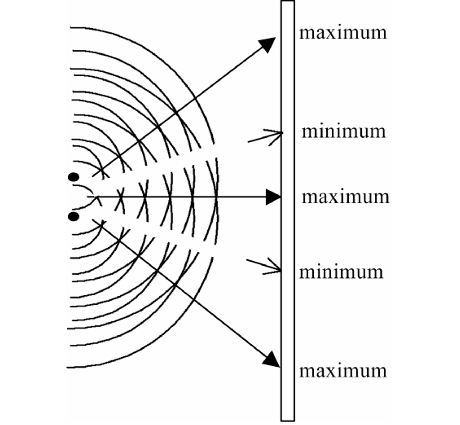
\includegraphics[height=0.22\textheight]{p3.png}
	\end{minipage}  
	\caption{光的干涉现象示意图\textsuperscript{\cite{4}}}
\end{figure}\par   
因为存在干涉现象时，反射光强度因干涉作用而存在周期性的减弱或增强，这种周期性的减弱或增强，在反射率随波数变化的曲线中，可以通过曲线的波动体现出来。所以对反射率与波数的测量数据进行分析，可以提取出干涉信号。在反射率随波数变化的曲线中存在波峰或波谷，波峰或波谷即对应干涉极值。\par 
通过已知数据分析，一定可以得到干涉振幅的两个极值，所以可以根据文献提供的相关公式\textsuperscript{\cite{3}}，直接计算干涉条纹极值的级数($\lambda_i$为第$i$个极值处的波长，$m$对应$\lambda_1$和$\lambda_i$的极数差,$k_i$对应第$i$个级数的波数)：\par 
\vspace{-1cm}
\begin{align}
	P_i=\dfrac{n\lambda_1}{\lambda_1-\lambda_i}+0.5
\end{align}\par 
根据光学相关知识，波长大小等于波数大小的倒数，可得下式：\par 
\begin{align}
\begin{cases}
	\lambda_1=\dfrac{1}{k_1}\\
	\lambda_i=\dfrac{1}{k_i}
	\label{e2}
\end{cases}
\end{align}\par 
根据上式，将干涉条纹极值级数计算公式中的波长转换为波数：\par 
\begin{align}
	P_i=\dfrac{m\dfrac{1}{k_1}}{\dfrac{1}{k_1}-\dfrac{1}{k_i}}+0.5=\dfrac{nk_i}{k_i-k_1}+0.5
\end{align}

三.外延层厚度计算模型\par 
根据文献提供的相关公式\textsuperscript{\cite{3}}，可以通过干涉条纹极值级数、入射角度、折射率等求解外延层厚度,求解时，得到的外延层厚度实际为第i个干涉条纹极值处的厚度：\par 
\begin{align}
	D_i=(P_i-0.5)\cdot\dfrac{1\lambda_i}{\sqrt{n_t^2-sin\theta_i^2}}+\dfrac{\Phi_A-\Phi_B}{2\pi}
\end{align}\par
其中$\Phi_A$、$\Phi_B$分别对应$A$、$B$两点的相位移,A、B两点位置如下图示意：\par 
\begin{figure}[H]
	\hspace{4cm}
	\begin{minipage}{0.3\textwidth}
		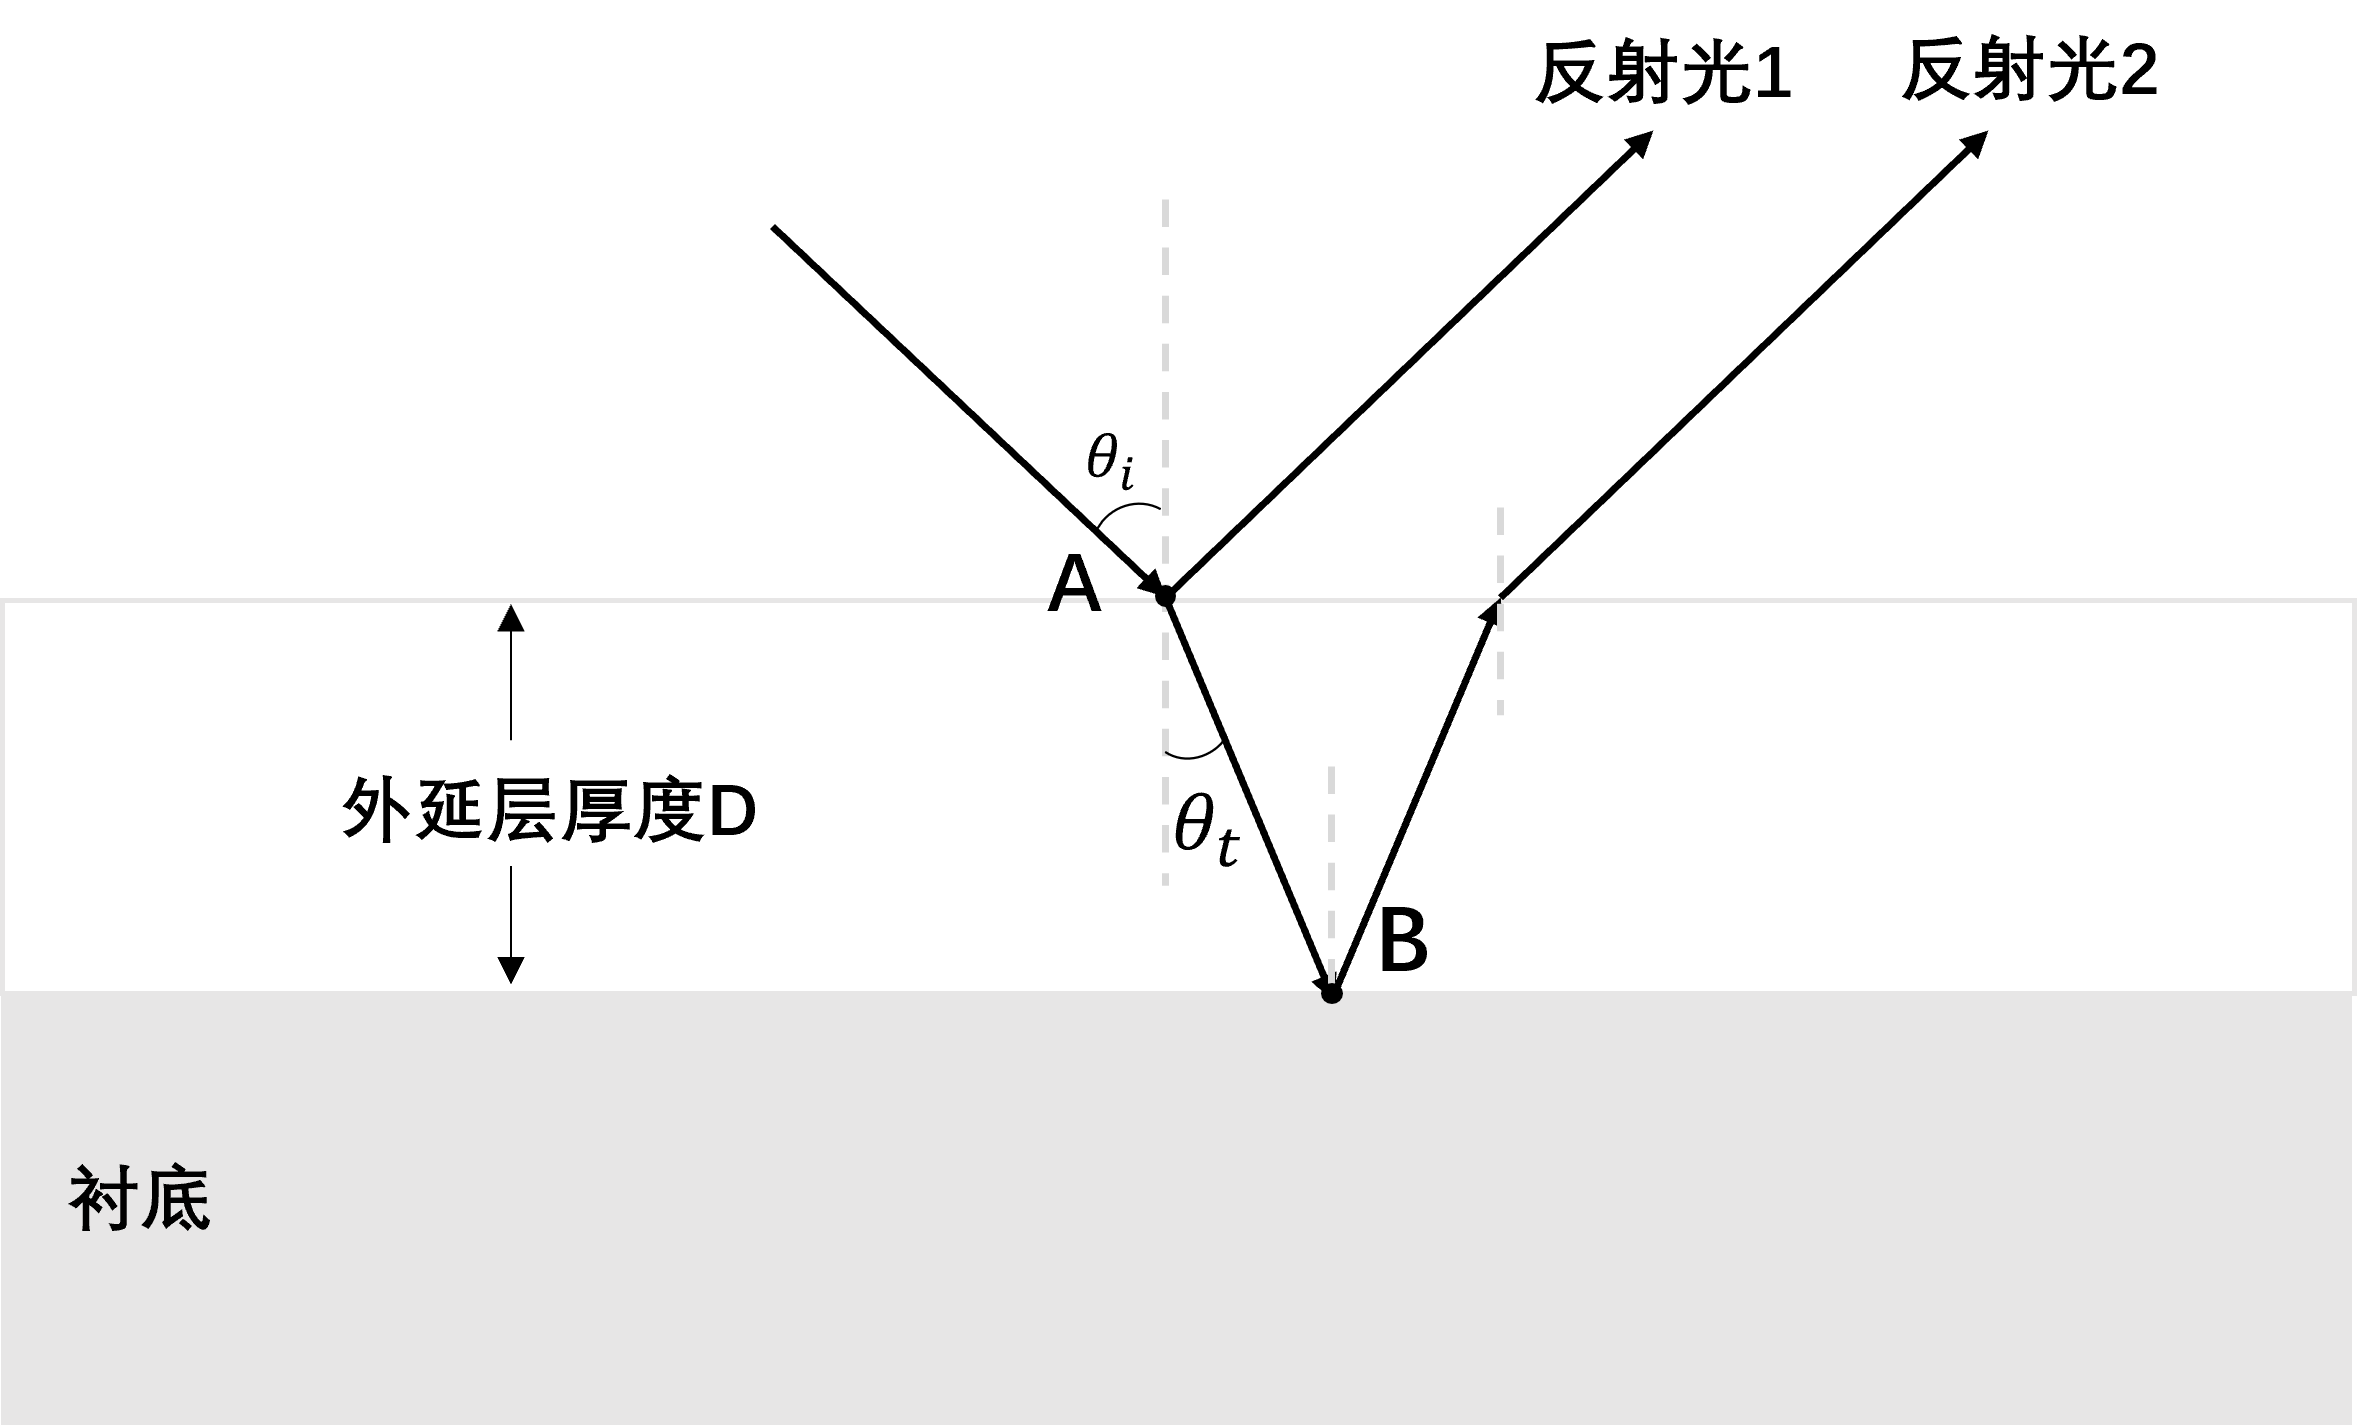
\includegraphics[height=0.23\textheight]{p2.png}
	\end{minipage}  
	\caption{A,B两点位置示意图}
\end{figure}\par   
 参考文献表明相位移部分数值结果极小，对厚度的计算结果影响体现在千分位上，可忽略不计：\par 
 \begin{align}
 	D_i=(P_i-0.5)\cdot\dfrac{1\lambda_i}{\sqrt{n_t^2-sin\theta_i^2}}
 \end{align}\par
 \subsubsection{模型展示}
 将干涉条纹极值级数计算模型代入外延层厚度计算模型：\par 
 \vspace{-1cm}
  \begin{align}
 	D_i=(\dfrac{nk_i}{k_i-k_1})\cdot\dfrac{\lambda_i}{\sqrt{n_t^2-sin\theta_i^2}}
 	\label{e1}
 \end{align}\par
 并根据公式(\ref{e2})，化简公式(\ref{e1})，得到化简后的外延层厚度计算公式：\par 
  \vspace{-1cm}
 \begin{align}
 	D_i=\dfrac{m}{k_i-k_1}\cdot\dfrac{1}{\sqrt{n_t^2-sin\theta_1^2}}
 \end{align}\par 
 将上式与折射率计算模型计算折射率进行结合，得到最终模型：\par 
 \begin{align}
 	\begin{cases}
 			D_i=\dfrac{m}{k_i-k_1}\cdot\dfrac{1}{\sqrt{n_t^2-sin\theta_1^2}}\\
 		\addlinespace
 		\addlinespace 
 			R=\dfrac{1}{2}[(\dfrac{\cos\theta_i-n_t\sqrt{1-(\dfrac{1}{n_t^2}(1-\cos\theta_i^2))}}{\cos\theta_i+n_t\sqrt{1-(\dfrac{1}{n_t^2}(1-\cos\theta_i^2))}})^2+(\dfrac{n_t\cos\theta_i-\sqrt{1-(\dfrac{1}{n_t^2}(1-\cos\theta_i^2))}}{n_t\cos\theta_i+\sqrt{1-(\dfrac{1}{n_t^2}(1-\cos\theta_i^2))}})^2]
 	\end{cases}
 \end{align}
\subsection{问题二：外延层厚度计算模型求解算法}
\subsubsection{求解准备}
1.原始数据分析\par 
首先，对附件1和附件2的原始数据进行可视化，以反射率为纵坐标，波数为横坐标，得到可视化结果如下：\par 
\begin{figure}[H]
	\hspace{0.75cm}
	\begin{minipage}{0.3\textwidth}
		\includegraphics[height=0.25\textheight]{附件1与附件2反射率对比图\_左右子图.eps}
	\end{minipage}  
	\caption{附件1(左)与附件2(右)反射率与波数数据关系对比展示图}
\end{figure}\par   
上图展示了不同入射角(附件1：$10^\circ$,附件2：$15^\circ$)情况下，反射率随波数变化对应的动态过程，其中左图对应的入射角度数为$10^\circ$的附件1数据，右图对应的入射角度数为$15^\circ$的附件2数据。由图可知，在固定的入射角大小下，反射率随着波数的增加波动变化，在波数为800左右和1000左右分别达到最大与最小值（排除0值）；在不同入射角情况下，反射率随波数变化而变化的规律一致，这一规律也与模型（反射率由外延层折射率和波数决定）完美契合。\par 
2.数据预处理\par 
由于实测反射率数据受测量误差与环境干扰影响，可能存在噪声。为更真实展现原始数据的变化趋势，采用了Savitzky-Golay滤波器进行处理，其原理是以51个数据点为一个窗口进行4阶多项式最小二乘拟合，用拟合值替换原始数据；参数设置上窗口大小为51（占总数据大小的0.68\%），以保留原始数据的趋势，采用4阶多项式以保留原始的非线性变化，不同入射角情况下的降噪前后变化图如下：\par 
\begin{figure}[H]
	\hspace{0.75cm}
	\begin{minipage}{0.3\textwidth}
		\includegraphics[height=0.26\textheight]{附件1与附件2降噪前后对比\_左右子图.eps}
	\end{minipage}  
	\caption{附件1(左)与附件2(右)反射率与波数数据降噪前后对比展示图}
\end{figure}\par   
上图中，灰色曲线为降噪前数据展示，蓝红曲线分别为附件1，2降噪后的曲线由数据降噪前后对应的折线图可知降噪处理后较好的保留了原始数据的变化趋势同时又减缓了噪声数据的影响。\par 
3.折射率求解准备\textsuperscript{\cite{10}}\par 
参考文献，取折射率计算公式中各光学参数值为：
\begin{table}[H]
	\caption{外延层厚度测算结果展示表}
	\centering
	\renewcommand{\tabcolsep}{50pt}
	\begin{tabular}{ccc}
		\toprule[1.5pt]
		光学参数名&参数大小&单位 \\
		\midrule[1pt]
		$\epsilon_{\infty}$ & 6.52 &  \\
		$\omega_{TO}$ & 793.9 & $cm^{-1}$ \\
		$\epsilon_{LO}$ & 970.1 & $cm^{-1}$ \\
		$\Gamma$ & 4.763 & $cm^{-1}$ \\
		$m^{\ast}$ & 0.42 & $m_o$ \\
		$\gamma$ & 757 & $cm^{-1}$ \\
		\bottomrule[1pt]
	\end{tabular}
\end{table}\par
\subsubsection{模型求解}
将附件数据中波数转化为相应光波角频率，并将角频率带入求解得到外延层的折射率\par
求解结果部分展示如下：\par
\begin{table}[H]
		\caption{折射率求解结果部分展示表}
	\centering
	\renewcommand{\tabcolsep}{9pt}
	\begin{tabular}{ccccc}
		\toprule[1.5pt]
	波数 ($cm^{-1}$) & 附件1反射率 (\%) & 附件1折射率 & 附件2反射率 (\%) & 附件2折射率  \\ 
		\midrule[1pt]
	399.6747  & 0.0000  & 3.2904  & 0.0000  & 3.2904   \\ 
	400.1569  & 31.2932  & 3.2910  & 36.3367  & 3.2910   \\ 
	400.6390  & 30.6043  & 3.2915  & 35.7521  & 3.2915   \\ 
	401.1211  & 29.9974  & 3.2920  & 35.1719  & 3.2920   \\ 
	401.6032  & 29.4148  & 3.2926  & 34.6691  & 3.2926   \\ 
	402.0853  & 28.9474  & 3.2931  & 34.1640  & 3.2931   \\ 
	402.5674  & 28.5645  & 3.2937  & 33.6644  & 3.2937   \\ 
	403.0496  & 28.2573  & 3.2942  & 33.1869  & 3.2942   \\ 
	403.5317  & 28.0509  & 3.2947  & 32.7582  & 3.2947   \\ 
	404.0138  & 27.9097  & 3.2953  & 32.3458  & 3.2953   \\ 
	404.4959  & 27.8248  & 3.2958  & 31.9616  & 3.2958   \\ 
		\bottomrule[1pt]
	\end{tabular}
\end{table}
二.波谷分析求解干涉条纹极值级数\par 
1.进行波谷分析求解的原因：\par 
在本题的场景中，对外延层厚度测算分析，条件满足反射光干涉相消的情况，干涉极值的曲线呈现为波谷型，所以进行波谷分析求解干涉极值。\par 
2.波谷分析求解的过程：\par 
基于降噪处理后的数据，通过代码实现，对反射率曲线中的极小值（谷值）进行检测，并统计波谷的数量以及每个波谷对应的波数值。待求的第$1$个级数的波数$k_1$以及第$m$个级数的波数$k_m$即为第一个波谷的波数以及第$m$个波谷的波数；待求解得极数差$n$即$m-1$表示波谷的序号差。\par 
波谷分析示意图如下：\par
\begin{minipage}{0.5\textwidth}
\begin{figure}[H]
	\hspace{-1cm}
	\begin{minipage}{0.3\textwidth}
		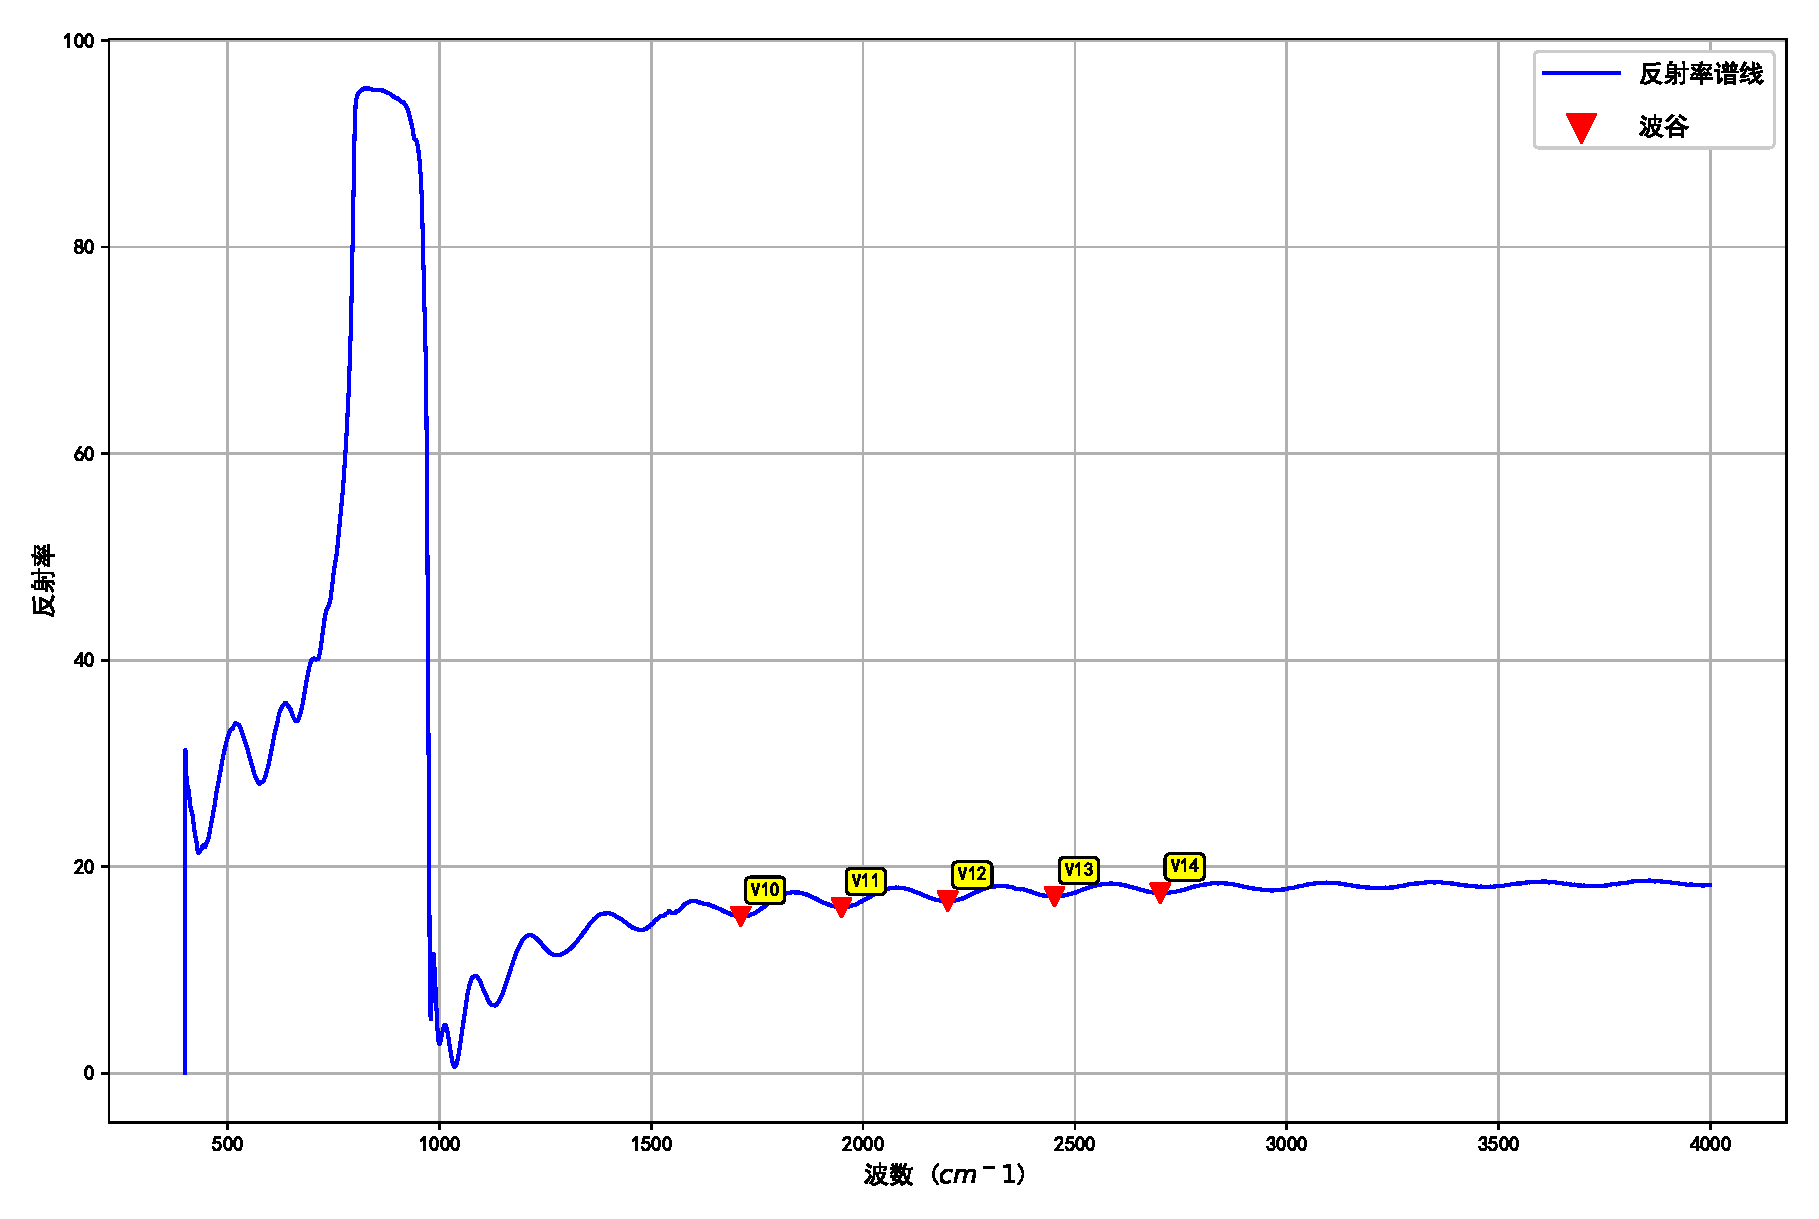
\includegraphics[height=0.24\textheight]{附件1波谷.eps}
	\end{minipage}  
	\caption{附件一反射率曲线波谷分析示意图}
\end{figure}
\end{minipage} 
\begin{minipage}{0.5\textwidth}
\begin{figure}[H]
\hspace{-0.75cm}
	\begin{minipage}{0.3\textwidth}
		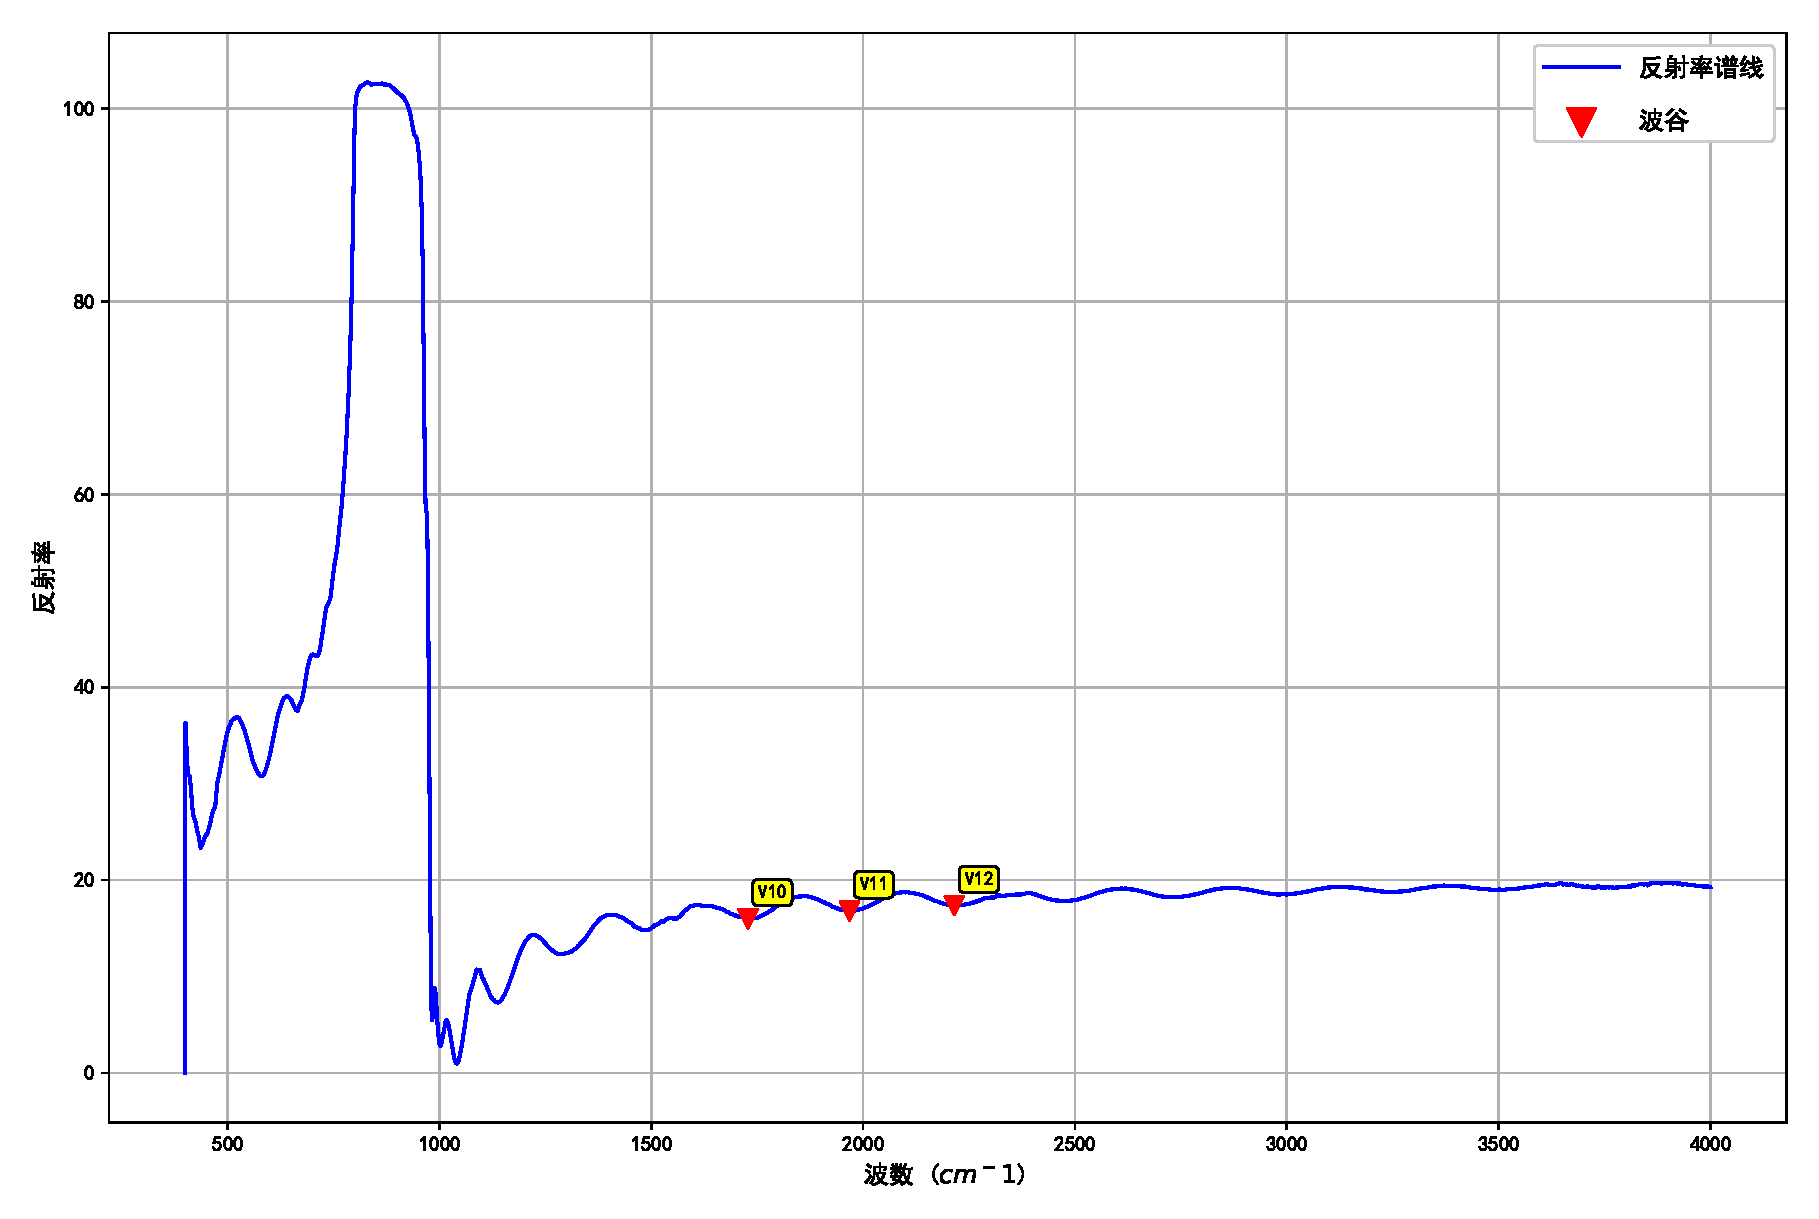
\includegraphics[height=0.24\textheight]{附件2波谷.eps}
	\end{minipage}  
	\caption{附件二反射率曲线波谷分析示意图}
\end{figure}
\end{minipage} 
观察上图，可将该SiC的反射率曲线大致分为： 低波数区域（$<500cm^{-1}$）、 反射率升高（$500–1000cm^{-1}$）、反射率降低（$1000–1500 cm^{-1}$）、 规律性震荡（$1500–3500 cm^{-1}$）、高频区域（$>3500 cm^{-1}$）五个部分。\par 
对这五个部分的曲线成因进行分析：\par 
1.低波数区域：无规律波动\par 
此区域通常对应远红外或太赫兹波段（长波长），碳化硅的声子（晶格振动）模式被激发。碳化硅是极性半导体，具有强的声子-光子耦合，可能形成声子极化激元（phonon-polaritons），导致反射率出现不规则振荡（尤其是靠近Reststrahlen波段边缘）。\par 
2.反射率升高：Reststrahlen波段\par 
碳化硅在远红外有一个典型的Reststrahlen波段（反射带），这是由于光学声子（横光学声子TO）与光子耦合导致的高反射平台。当入射光频率接近横光学声子频率（TO phonon）时（，介电函数虚部增大，实部变为负值，导致高反射（通常>80\%），图中反射率在$700–1000cm^{-1}$之间升高，正是Reststrahlen效应的体现。Reststrahlen波段，也称为剩余射线带，在这个波段内，材料会表现出非常高的反射率，且光子的能量会被晶格振动剧烈地吸收，这种强烈的共振吸收会导致材料的介电函数（$\epsilon(v)$） 发生巨大变化。当介电函数的实部 $\epsilon_{1} < 0$ 时，材料的光学行为会类似于金属即对光具有高反射率。在两个频率之间（v\_TO < v < v\_LO），材料表现出高反射性。低于v\_TO或高于v\_LO，ε₁ > 0，材料变得更透明，反射率迅速下降。\par 
3. 反射率降低：Reststrahlen波段边缘\par 
超过Reststrahlen波段后，介电函数实部由负变正，材料从类金属行为（高反射）转变为介电行为（透明或吸收）。反射率下降是因为光子能量逐渐超过光学声子能量，晶格振动无法响应，材料开始变得透明（对红外透明），反射率下降。此时若红外光远离波段且在 v\_LO 频率附近，$\epsilon_{1}$ 从负值快速增加并通过零，必然会经过 $\epsilon_{1} = 1$ 的这个点。当 $\epsilon_{1} = 1$ 时，折射率 $n = 1$，恰好与空气匹配，即此时出现反射率几乎为0的情况。\par 
4.规律性震荡：法布里-珀罗干涉\par 
此区域出现规律振荡，这是典型的法布里-珀罗干涉（Fabry-Perot interference）现象。当碳化硅样品为薄层或具有平行表面时，入射光在上下界面间多次反射并发生干涉，形成振荡条纹。\par 
振荡周期$\Delta ν$与样品厚度$d$满足(其中$n$为折射率)：\par 
\begin{align}
\Delta v=\dfrac{1}{2nd}
\end{align}\par 
5.高频区域：反射率平稳\par 
在更高波数（短波长，近红外/可见光），光子能量远高于声子能量，晶格振动不再影响光学响应。此时反射率由电子跃迁（带间吸收）决定。碳化硅是宽带隙半导体（$Eg\approx3.2 eV for 4H-SiC$），在红外波段无电子吸收，因此反射率趋于平稳（主要由表面菲涅尔反射决定，折射率$n\approx2.6$，反射率约20\%）。
最终选择的波数段为规律性震荡（$1500–3500 cm^{-1}$）作为干涉条纹分析求解外延层厚度时的波谷分析范围。\par 
选用规律性震荡（$1500–3500 cm^{-1}$）波数段的原因:\par 
(1)高信噪比，振荡清晰：在这个区域，干涉条纹的对比度（振幅）高且周期性非常规则。这使得准确判断波峰或波谷的位置非常容易，减小了读数误差。\par 
(2)材料透明，吸收可忽略：这是最重要的原因。在此波数范围，光子能量远高于碳化硅的声子能量（Reststrahlen波段已结束），因此消光系数 $κ \approx 0$，材料几乎无吸收。\par 
这意味着折射率$ n$ 是一个实数，并且变化平缓（色散较弱）。公式 $\Delta ν̄ = \dfrac{1}{2nd}$在此处严格成立。\par 
如果存在吸收（$k> 0$），会引入额外的相位偏移，使得振荡峰位移动，导致公式失效，计算结果不准。\par 
折射率行为稳定：在透明区域，碳化硅的折射率 $n$ 主要来自电子极化贡献，随波数变化非常缓慢（近乎一个常数）。你可以使用一个单一的平均折射率值（例如 $n \approx 2.6$）来进行计算，而不必担心它随波数剧烈变化。\par 
远离特征吸收边：此区域远离了Reststrahlen波段和可能的电子吸收边（对于SiC，电子吸收边在可见光/紫外区），避免了这些强烈色散区对振荡行为的复杂影响。\par 
3.求解结果：\par 
以附件一10项波谷数据为例：求解得到第$1$个级数的波数$k_1$以及第$10$个级数的波数$k_10$分别为：$433.4229cm^{-1}$和$1948.7160 cm^{-1}$。极数差$n$为：。\par 
三.外延层厚度求解\par 
将求解得到的数据代入公式，求解得到波谷处的外延层厚度的测算结果：\par 
\begin{table}[H]
	\caption{外延层厚度测算结果展示表}
	\centering
	\renewcommand{\tabcolsep}{25pt}
	\begin{tabular}{ccccc}
		\toprule[1.5pt]
	 ~ & 波数 & 反射率 & 折射率 & 厚度 ($\mu m$) \\ 
		\midrule[1pt]
	附件1 & 2199.8980  & 16.6694  & 2.4573  & 16.3184   \\ 
	~ & 2451.5630  & 17.1079  & 2.4786  & 16.1780   \\ 
	~ & 2701.3000  & 17.4453  & 2.4932  & 16.0827 \\ 
	均值 & 2450.9203  & 17.0742  & 2.4764  & 16.1930  \\ 
 
	附件2& 1967.5180  & 16.8041  & 2.4279  & 16.9932   \\ 
	~ & 2215.3260  & 17.3621  & 2.4589  & 16.7778  \\ 
	均值 & 1970.2500  & 16.7177  & 2.4219  &17.0384   \\ 
		\bottomrule[1pt]
	\end{tabular}
\end{table}
\subsection{问题三：多光束干涉下外延层厚度计算模型}
\subsubsection{多光束干涉必要条件\textsuperscript{\cite{7}}}
干涉的必要条件：\par 
1.叠加光波相位差固定不变\par 
根据干涉现象的定义，干涉现象是光束叠加在一定区域形成有明条纹和暗条纹分布的现象。而在光束叠加的时候，要形成稳定的干涉条纹，叠加区域内不同的点光强必须不同，而光强不一样是因为位相差不一样。而要让不同点因位相差不同产生稳定的光强差异，就必须满足叠加光波的相位差固定不变，否则无法进行比较，也就是说无法产生稳定的干涉现象。\par 
2.	叠加光波的振动方向相同\par 
叠加光波的振动方向影响光的叠加效果，只有在振动方向相同时，光矢量才可以在同方向叠加，合光强就不等于两束光光强的简单相加，因相位差不同，出现光强的强弱分布，形成明暗现象，也就是干涉现象。若振动方向垂直，光束无法在同方向上进行叠加增强或减弱，也就无法因位相差不同形成干涉现象。\par 
3.	叠加光波的频率相同\par 
光波的频率决定光波的相位随时间变化的速度，若两束光波的频率不一致，则两束光波相位变化速度不一致，两束光波的相位差就不可能是固定不变的，而是随时间会发生变化的，不满足"叠加光波相位差固定不变"这一必要条件，则一定不能实现干涉现象。所以要实现干涉现象一定要满足叠加光波的频率相同。\par 
4.相干长度大于光程差\par 
相干长度表示两束光能够始终保持相对稳定的相位关系的光程差范围，光程差表示两束光的传播光程的差值。只有当相干长度大于光程差时，两束光才更有可能来自同一波列，或者具有固定相位关系的波列片段，才能保证在叠加区域内，叠加光波相位差固定不变，满足产生稳定干涉现象的必要条件。保证相干长度大于光程差才能保证稳定的干涉现象产生。\par
多光束干涉现象的必要条件 ：\par 
1.	反射率应比较大\par 
只有反射率较大，后续反射得到的光束光强才足够大，只有后续光束的光强足够大，才可以进行光强差异分析，才会有明显的光强差异分布，形成稳定的干涉条纹。证明过程如下\textsuperscript{\cite{7}}：\par 
假设在红外光光源的光线射入外延层时，入射光振幅为$A$,反射系数为$r$，透射系数为$t$，自外延层射出至环境中的反射光线对应的反射系数设为$r'$,透射系数设为$t'$。那么从外延层反射出来的各光束的振幅依次为：\par 
\begin{align}
	rA,tt'rA,tt'r'^3A,tt'r'^5A...
	\label{e3}
\end{align}\par 
通过菲涅尔公式可以证明$r$，$t$，$r'$,$t'$满足下式关系：\par 
\begin{align}
	r=-r',tt'=1-r^2
	\label{e5}
\end{align}\par 
而$r$，$t$，$r'$,$t'$与外延层表面反射率$R$和透射率$T$之间满足关系：\par 
\begin{align}
	r^2=r'^2=R,tt'=1-R=T
	\label{e6}
\end{align}\par 
根据光强计算公式得到各反射光束的光强与外延层表面反射率与透射率关系如下：\par 
\begin{align}
	\begin{cases}
		I_1=r^2=R\\
		I_2=(tt'r')^2=T^2R\\
		I_3=(tt'r^3)^2=T^2R^3\\
		I_4=(tt'r^5)^2=T^2R^5
		\label{e4}
	\end{cases}
\end{align}\par 
由于光在介质中透射会有能量损耗，透射率$T$通常小于 1,随着反射光束的顺序往后，光强表达式中 R 的幂次不断升高，反射率 R 对光强的 “放大”作用会以类似指数增长的态势体现出来\textsuperscript{\cite{5}}。所以只有反射率较大，后续反射得到的光束光强才足够大。\par
2.干涉条纹的对比度应较高\par 
若条纹对比度低，则条纹会模糊，无法进行光程差测量以及光谱分析，失去外延层厚度测量的实用价值。\par 
\subsubsection{多光束干涉对计算精度影响\textsuperscript{\cite{8}}} 
对于所获取的干涉条纹数据，必须首先进行相位提取以计算其波前相位。因为无论使用哪种相位提取算法，都需要借助反正切函数来获取波前相位分布，反正切函数具有周期性，其值域为$[-\pi,\pi]$，所以相位值会以 2$\pi$为周期重复。当多光束干涉时会形成多个干涉条纹，意味着光程差的变化跨越了多个周期，其对应的相位分布也会跨越多个周期，导致相邻周期处因周期限制，出现 2π 的跳变 ，即从$\pi\to-\pi$。显然，这种现象导致多光束干涉的情况无法反映, 外延层真实的表面形状信息。降低根据多光束干涉现象进行测算的Si外延层厚度的精度。\par 
\subsubsection{硅晶圆片测试数据多光束干涉判断}
1.满足干涉条纹的对比度应较高条件证明：\par 
根据光学相关知识，条纹对比度计算公式如下($I_{max},I_{min}$分别代表最大光强和最小光强)：\par 
\begin{align}
	k=\dfrac{I_{max}-I_{min}}{I_{max}+I_{min}}
\end{align}\par 
由于未知外延层折射率以及厚度情况，故暂时无法通过爱里公式求解计算光强；且对比度的分析关注光强的相对变化程度，而不是绝对光强的具体数值，所以可以通过反射率简化分析，刻画这种相对变化。采用反射率来反应光照强度,定义对比度k计算公式如下：\par 
\begin{align}
	k=\dfrac{R_{max}-R_{min}}{R_{max}+R_{min}}
\end{align}\par 
将附件3、4原始数据带入可以得到两种入射角情况下的对比度分别为0.996638和0.992393对比度接近于1，满足干涉条纹的对比度应较高这一必要条件，认为可能符合多光束干涉。\par 
2.满足反射率应比较大条件证明\par 
对附件3和附件4的测试结果绘制反射率数据的频率分布直方图：\par 
\begin{figure}[H]
	\hspace{1cm}
	\begin{minipage}{0.3\textwidth}
		\includegraphics[height=0.28\textheight]{附件3与附件4反射率频率直方图对比\_左右子图.eps}
	\end{minipage}  
	\caption{附件3(左)与附件4(右)反射率频率直方图}
\end{figure}\par 
统计数据信息结果如下：\par 
\begin{table}[H]
	\caption{附件3(左)与附件4(右)反射率数据统计展示表}
	\centering
	\renewcommand{\tabcolsep}{21pt}
	\begin{tabular}{cccccc}
		\toprule[1.5pt]
	  ~ & 样本数 & 均值 & 标准差 & 最小值 & 最大值  \\ 
		\midrule[1pt]
		附件3 &  7469 &  32.0997 &  13.4164 &  0.0000 &  79.8020  \\ 
	附件4 &  7469 &  35.3517 &  15.0175 &  0.0000 &  91.4894  \\ 
		\bottomrule[1pt]
	\end{tabular}
\end{table}
根据上述信息，分析附件3和附件4的测试结果，得到的反射率主要分布在30\%左右，反射率相对较大，故可能存在多光束干涉。\par 
3.满足叠加光波相位差固定不变条件检验\par 
前后两束反射光的总相位差$\phi$由光程差导致的相位差$\phi_g$和界面反射相移导致的相位差$\phi_f$两部分构成，即：\par 
\begin{align}
	\phi=\phi_g+\phi_f
\end{align}\par 
以第二第三束光为例进行分析：\par 
绘制光的传播路径及相关符号标识示意图如下：\par 
\begin{figure}[H]
	\hspace{3cm}
	\begin{minipage}{0.3\textwidth}
		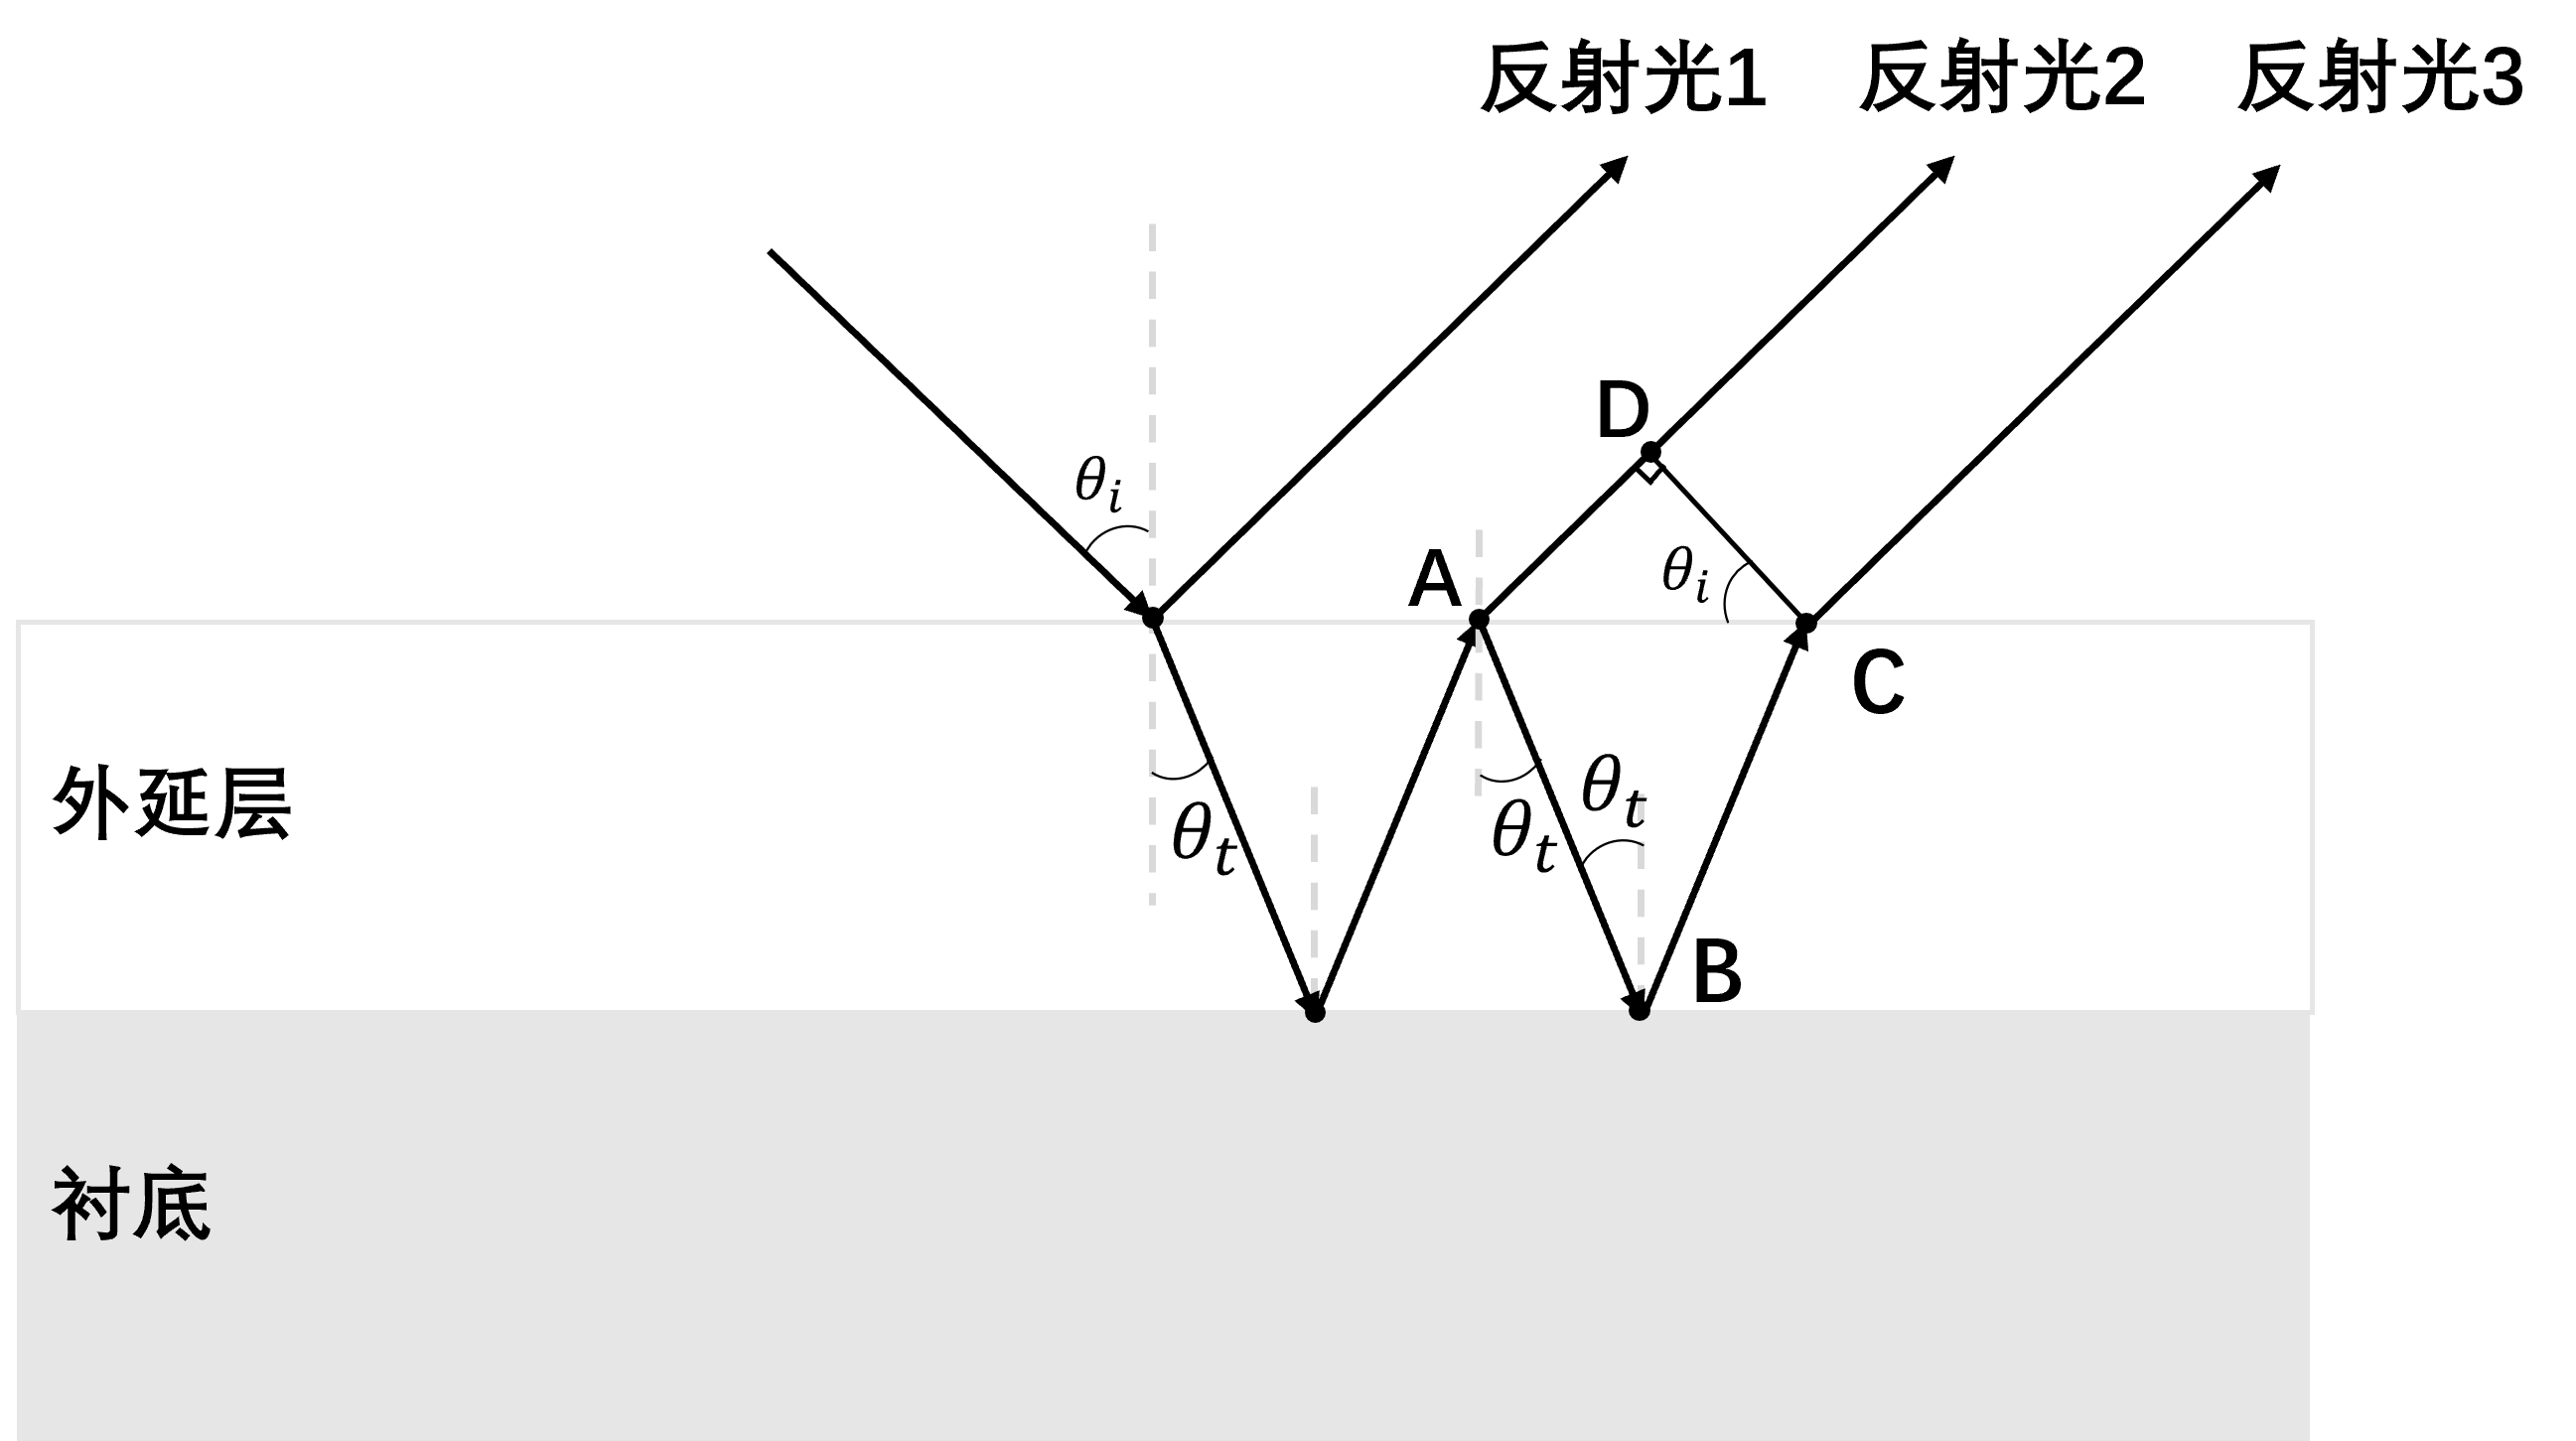
\includegraphics[height=0.3\textheight]{p4.png}
	\end{minipage}  
	\caption{光的传播路径示意图}
\end{figure}\par 
(1)光程差导致的相位差$\phi_g$计算方程如下（将距离统一转化为光在环境传播的有效距离, $n_t$为外延面折射率，$L_{AB}$、$L_{BC}$和$L_{AD}$分别对应$A$到$B$，$B$到$C$以及$A$到$D$之间的距离）：\par 
\begin{align}
	\phi_g=\dfrac{2\pi}{\lambda}\cdot (n_t(L_{AB}+L_{BC})-L_{AD})
\end{align}\par 
其中关于$L_{AB},L_{BC}$的计算，根据对称性以及其水平方向上的关系可知$L_{AB},L_{BC}$满足下式(D为外延层厚度)：\par 
\begin{align}
	L_{AB}=L_{BC}=\dfrac{D}{cos\theta_t}
\end{align}\par 
由示意图可知$L_{AD}$满足以下公式：\par 
\begin{align}
	L_{AD}=L_{AC}\sin\theta_i=2L_{AB}\sin\theta_t\sin\theta_i=2D\tan\theta_t\sin\theta_i
\end{align}\par 
(2)界面反射相移导致的相位差$\phi_f$对应计算公式($\Phi_2$、$\Phi_3$分别对应第二和第三束光的相位移)：\par
\begin{align}
	\phi_f=\Phi_2-\Phi_3
\end{align}\par 
硅晶体衬底通常是单晶硅，其结构规整，原子排列有序。而外延层是在衬底上通过气相沉积等技术生长的一层硅材料。总体而言，环境的折射率小于外延层折射率小于衬底的折射率。由于红外光以小入射角$10^\circ$射入，根据斯涅尔定律$n_i\ast sin\theta_i=n_t\ast sin\theta_t$可知，折射角小于$10^\circ$，而对应外延层-衬底界面将以更小的入射角射入\textsuperscript{\cite{5}}。\par 
当小角度从光疏介质射向光密介质反射时，反射光会产生$\pi$的相位差（半波损失），而从光密介质射向光疏介质反射时，反射光不会产生相位差。对于第二束光，存在一次从光疏介质射向光密介质的反射，相位移为$\pi$；对于第三束光，有两次从光疏介质射向光密介质的反射，一次从光密介质射向光疏介质的反射，总相位移为2$\pi$，故反射导致的总相位差$\phi_f$为$-\pi$\textsuperscript{\cite{6}}。\par 
(3)综上，得到第二三束光的总相位差计算公式如下：\par 
\begin{align}
	\phi=\dfrac{2\pi}{\lambda}\cdot(n_t\dfrac{2D}{\cos\theta_t}-2D\tan\theta_t\sin\theta_i)-\pi
\end{align}\par 
根据总相位差公式推导过程分析，光束的选择（计算那一组临近的光束总相位差）不影响光程差导致的相位差$\phi_g$，而在界面反射相移导致的相位差$\phi_f$始终保持固定的相位差值，所以满足叠加光波相位差固定不变条件，可能存在多光束干涉。\par 
4.满足叠加光波的频率相同条件检验\par 
在本文中进行外延层厚度测算时，使用的是红外光源。红外光在反射过程中光子的波长及能量不变，仅仅改变传播方向；红外光在透射过程中其速度与波长发生改变，而频率并不变。反射和透射这两个过程属于弹性散射过程，光子的能量均不发生变化，根据能量和频率之间的计算公式$E=h\upsilon$（$h$为普朗克常数）可知光子的频率也不发生改变，前后两束光的频率一致。\par 
\subsubsection{附件1，2数据中出现多光束干涉证明}
\subsubsection{多光束外延层厚度计算模型建立}
一.硅晶圆片外延层厚度计算模型\par 
1.硅晶体折射率求解模型\par 
在折射率求解模型建立上，分别从两个经验公式搭建，各自求解折射率，相互比较验证。\par 
(1)Herzberger-type色散经验公式：\par 
\begin{align}
	n_t=A+BL+CL^2+D\lambda^2+E\lambda^4
\end{align}\par 
其中$lambda$为波长，单位为微米，参数$L$计算公式如下(0.028为14种材料（包括硅）在短波长下折射率突变上升的平均渐近线的平方):\par 
\begin{align}
	L=\dfrac{1}{\lambda^2-0.028}
\end{align}\par 
根据参考文献指出的波长范围满足$1.12-588$微米时，经验公式的系数取值如下：\par 
\begin{align}
	\begin{cases}
		A=3.41906\\
		B=1.23172\times 10^{-1}\\
		C=2.65456\times 10^{-2}\\
		D=-2.66511\times 10^{-8}\\
		E=5.45852\times 10^{-14}
	\end{cases}
\end{align}\par 
(2)Sellmeier-type 色散经验公式:\par 
\begin{align}
	n_t^2=\varepsilon+\frac{A}{\lambda^2}+\dfrac{B\lambda_1^2}{\lambda^2-\lambda_1^2}
\end{align}\par 
其中$\lambda$为波长，单位为微米，,参数根据文献已知数据如下：\par 
\begin{align}
	\begin{cases}
		\lambda_1=1.1071\mu m\\
		\varepsilon=1.6858\times{10}^{-1}\\
		A=9.39816\times{10}^{-1}\\
		B=8.10461\times{10}^{-3}
	\end{cases}
\end{align}\par 
2.外延层厚度求解模型\par 
(1)总反射率函数推导：\par 
根据公式(\ref{e3})-(\ref{e4})可以求解得到多光束干涉汇合时的电磁波电场表达式(其中$\omega$是光波的角频率，$\delta_0$是位相常数)：\par 
\begin{align}
	\begin{cases}
		E_1^{(r)}=rA^{(i)}\times e^{i(\delta_0-\omega t)}\\
		E_2^{(r)}=r^\prime tt^\prime A^{(i)}\times e^{i(\delta_0+\delta-\omega t)}\\
		E_3^{(r)}=r^{\prime3}tt^\prime A^{(i)}\times e^{i(\delta_0+2\delta-\omega t)}\\
		E_4^{(r)}=r^{\prime5}tt^\prime A^{(i)}\times e^{i(\delta_0+3\delta-\omega t)}\\
		\label{e7}
	\end{cases}
\end{align}\par 
舍弃共同因子$e^{i(\delta_0-\omega t)}$，得到合成场的复振幅为:\par 
\begin{align}
	A^{(r)}&=(r+tt^\prime r^\prime e^{(i\delta)}+tt^\prime{r^\prime}^3e^{(i2\delta)}+tt^\prime r^\prime e^{(i3\delta)}+\ldots)A^{(i)}\\
	&=(r+tt^\prime r^{\prime e^{(i\delta)}}[1+r^{\prime2}e^{(i\delta)}+r^{\prime4}e^{(i2\delta)}+\ldots])A^{(i)}
	\label{e8}
\end{align}\par 
上式方括号内是一个递降等比级数，当外延层足够长时，反射光束数目很大；当光束数量趋于无穷大的极限情况下，得到下式：\par 
\begin{align}
	A^{(r)}=(r+\dfrac{\ tt^\prime r\prime e^{i\delta}}{1-r^{\prime2}e^{i\delta}})A^{(i)}
\end{align}\par 
由前文中给出的公式(\ref{e5})，(\ref{e6})变形得到总反射率$R_t$、外延层表面反射率$R$、位相差$\delta$之间的关系式：\par 
\begin{align}
	R_t&=(\dfrac{A^{(i)}}{A^{(i)}})^2=(\sqrt{R}+\dfrac{\ tt^\prime \sqrt{R}^{\prime e^{i\delta}}}{1-\sqrt{R}^{\prime2}e^{i\delta}})^2=(\dfrac{\sqrt{R}-\sqrt{R}Re^{i\delta}+(1-R)\sqrt{R}\prime e^{i\delta}}{1-Re^{i\delta}})^2\\
	&=(\dfrac{\sqrt{R}-\sqrt{R}Re^{i\delta}+\sqrt{R}^\prime e^{i\delta}-\sqrt{R}^\prime R e^{i\delta}}{1-Re^{i\delta}})^2=(\dfrac{\sqrt{R}+\sqrt{R}^\prime e^{i\delta}}{1-Re^{i\delta}})^2=(\dfrac{\sqrt{R}-\sqrt{R}e^{i\delta}}{1-Re^{i\delta}})^2
	\label{e9}
\end{align}\par 
在外延层表面反射率$R$的计算上，进行如下推导，得到与折射率相关的表达式：\par 
根据描述折射率与反射率间关系的公式：菲涅耳公式(Fresnel equation)\textsuperscript{\cite{1}}，得到振幅系数$r$的求解方程如下($\theta_i$对应入射角，$\theta_t$对应折射角，$n_i$对应环境折射率，$n_t$对应外延面折射率)：\par 
\begin{align}
	\begin{cases}
		r_s=\dfrac{n_i\cos\theta_i-n_t\cos\theta_t}{n_i\cos\theta_i+n_t\cos\theta_t}\\
		r_p=\dfrac{n_t\cos\theta_i-n_i\cos\theta_t}{n_t\cos\theta_i+n_i\cos\theta_t}\\
	\end{cases}
\end{align}\par 
由于非偏振光的反射率$R$的计算取决于射入光线的$p$和$s$偏振，且非偏振光的反射率R可由$R_S$和$R_p$的均值求解（$R_S$、$R_p$分别对应垂直和平行偏振平面的反射率）：\par  
\begin{align}
	R=\dfrac{(R_S+R_p)}{2}=\dfrac{(r_s^2+r_p^2)}{2}
\end{align}\par 
由斯涅尔定律可知入射角和反射角满足方程：\par 
\begin{align}
	n_i\cdot sin\theta_i=n_t\cdot sin\theta_t
\end{align}\par 
为计算折射角对上式变形：\par 
\begin{align}
	\cos\theta_t=\sqrt{1-(\dfrac{n_i}{n_t}sin\theta_i)^2}=\sqrt{1-({\dfrac{n_i}{n_t}}^2(1-cos\theta_i^2))}
\end{align}\par 
环境折射率$n_i$为1，将相关参数带入，得到折射率与反射率的关系表达式：\par 
\begin{align}
	R=\dfrac{1}{2}[(\dfrac{\cos\theta_i-n_t\sqrt{1-(\dfrac{1}{n_t^2}(1-\cos\theta_i^2))}}{\cos\theta_i+n_t\sqrt{1-(\dfrac{1}{n_t^2}(1-\cos\theta_i^2))}})^2+(\dfrac{n_t\cos\theta_i-\sqrt{1-(\dfrac{1}{n_t^2}(1-\cos\theta_i^2))}}{n_t\cos\theta_i+\sqrt{1-(\dfrac{1}{n_t^2}(1-\cos\theta_i^2))}})^2]
	\label{e10}
\end{align}\par 
(2)位相差$\delta$计算公式如下：\par 
\begin{align}
	\delta=\dfrac{4\pi}{\lambda}n_tDcos\theta_i
	\label{e11}
\end{align}\par 
(3)综上建立关于总反射率的外延层厚度求解模型:
\begin{align}
	\begin{cases}
		R_t=(\dfrac{\sqrt{R}-\sqrt{R}e^{i\delta}}{1-Re^{i\delta}})^2=R(\dfrac{1-e^{i\delta}}{1-Re^{i\delta}})^2 \\
		\delta=\dfrac{4\pi}{\lambda}n_tDcos\theta_i\\
		R=\dfrac{1}{2}[(\dfrac{\cos\theta_i-n_t\sqrt{1-(\dfrac{1}{n_t^2}(1-\cos\theta_i^2))}}{\cos\theta_i+n_t\sqrt{1-(\dfrac{1}{n_t^2}(1-\cos\theta_i^2))}})^2+(\dfrac{n_t\cos\theta_i-\sqrt{1-(\dfrac{1}{n_t^2}(1-\cos\theta_i^2))}}{n_t\cos\theta_i+\sqrt{1-(\dfrac{1}{n_t^2}(1-\cos\theta_i^2))}})^2]\\
		n_t=3.41\\
\end{cases}
\end{align}\par
二.碳化硅晶圆片外延层厚度计算模型\par 
参考公式(\ref{e7})、(\ref{e8})求解得到在双光束干涉条件下的复振幅度为：\par 
\begin{align}
	A^ {(r)}=(r+tt'r'e^{i\sigma})A^{(i)}
\end{align}\par 
由该公式可以求解在双光束干涉条件下的总反射率为：\par 
\begin{align}
	R_t=(\dfrac{A^{(r)}}{A^{(i)} }  )^2=(r+tt'r'e^{i\sigma})^2=(r+(1-R)\cdot(-r) e^{i\sigma}  )^2=R(1+(R-1)e^{i\sigma} )^2
\end{align}\par 
将公式(\ref{e9})进行转化可以求解得到在多光束干涉条件下的总反射率为：\par 
\begin{align}
	R_t=(\dfrac{\sqrt{R}-\sqrt{R} e^{i\sigma}}{1-Re^{i\sigma}})^2=R(1+\dfrac{Re^{i\sigma} -e^{i\sigma}  }{1-Re^{i\sigma}  })^2=R(1+\dfrac{1}{1-Re^{i\sigma} }(R-1)e^{i\sigma} )^2
\end{align}\par 
这两个公式可以看出当多光束干涉存在而仅仅将其简化考虑为双光束干涉时，由于双光束缺少了$\dfrac{1}{1-Re^{i\sigma}}$这个补偿项，从而影响了前文求解外延层厚度的求解，故为提高厚度求解的精度，应减少补偿项带来的精度变化即尽量使$Re^{i\sigma}$趋于0,界面反射率R求解可参考公式(\ref{e10})，而$\delta$的求解参考公式(\ref{e11})。\par 
\subsubsection{多光束外延层厚度计算模型求解}
一.硅晶圆片外延层厚度求解\par 
在已知总反射率的外延层厚度求解模型，需要求解模型中的外延层厚度D。对此采用非线性的最小二乘法对外延层厚度进行求解。\par
非线性最小二乘法是一种用于估计非线性模型参数的优化方法，核心是通过迭代调整外延层厚度使得计算出来的总发射率与附件检测得到的发射率之间的残差平方和最小化。核心公式：\par 
\begin{align}
	min\sum_{i=1}^{n}[R_{t\ i}-f(D)]^2
\end{align}\par 
其中$R_{t\ i}$为$i$波数下总发射率检测值，$f(D)$为外延层厚度为$D$情况下的总发射率理论值，最小二乘法通过迭代找出最小残差平方和得到相应的外延层厚度$D$。\par 
计算拟合效果评价指标均方误差(MSE)和均方根误差(RMSE)结果展示如下：\par 
\begin{table}[H]
	\caption{拟合效果评价指标展示表}
	\centering
	\renewcommand{\tabcolsep}{50pt}
	\begin{tabular}{cc}
		\toprule[1.5pt]
		 均方误差 (MSE) & 均方根误差 (RMSE)  \\ 
		\midrule[1pt]
			0.9759353 & 0.987894  \\ 
		\bottomrule[1pt]
	\end{tabular}
\end{table}
求解得到附件3，4的外延层厚度为：$4.7577\mu m$和$  4.5593\mu m$。
二.碳化硅晶圆片外延层厚度求解\par 
由图可知当R不断减小的过程中，多光束干涉和双光束干涉之间的反射率差异不断降低，而通过R的计算公式可知，当入射角固定的情况下，折射率$n_t$相对较小时对应的界面反射率也相对较小，多光束干涉的影响也越小，对此在总反射率相对稳定后，取折射率相对较低的极小值算厚度，即通过波数较小部分对应的波束差来算取外延层厚度。\par 
\begin{figure}[H]
	\hspace{2cm}
	\begin{minipage}{0.6\textwidth}
		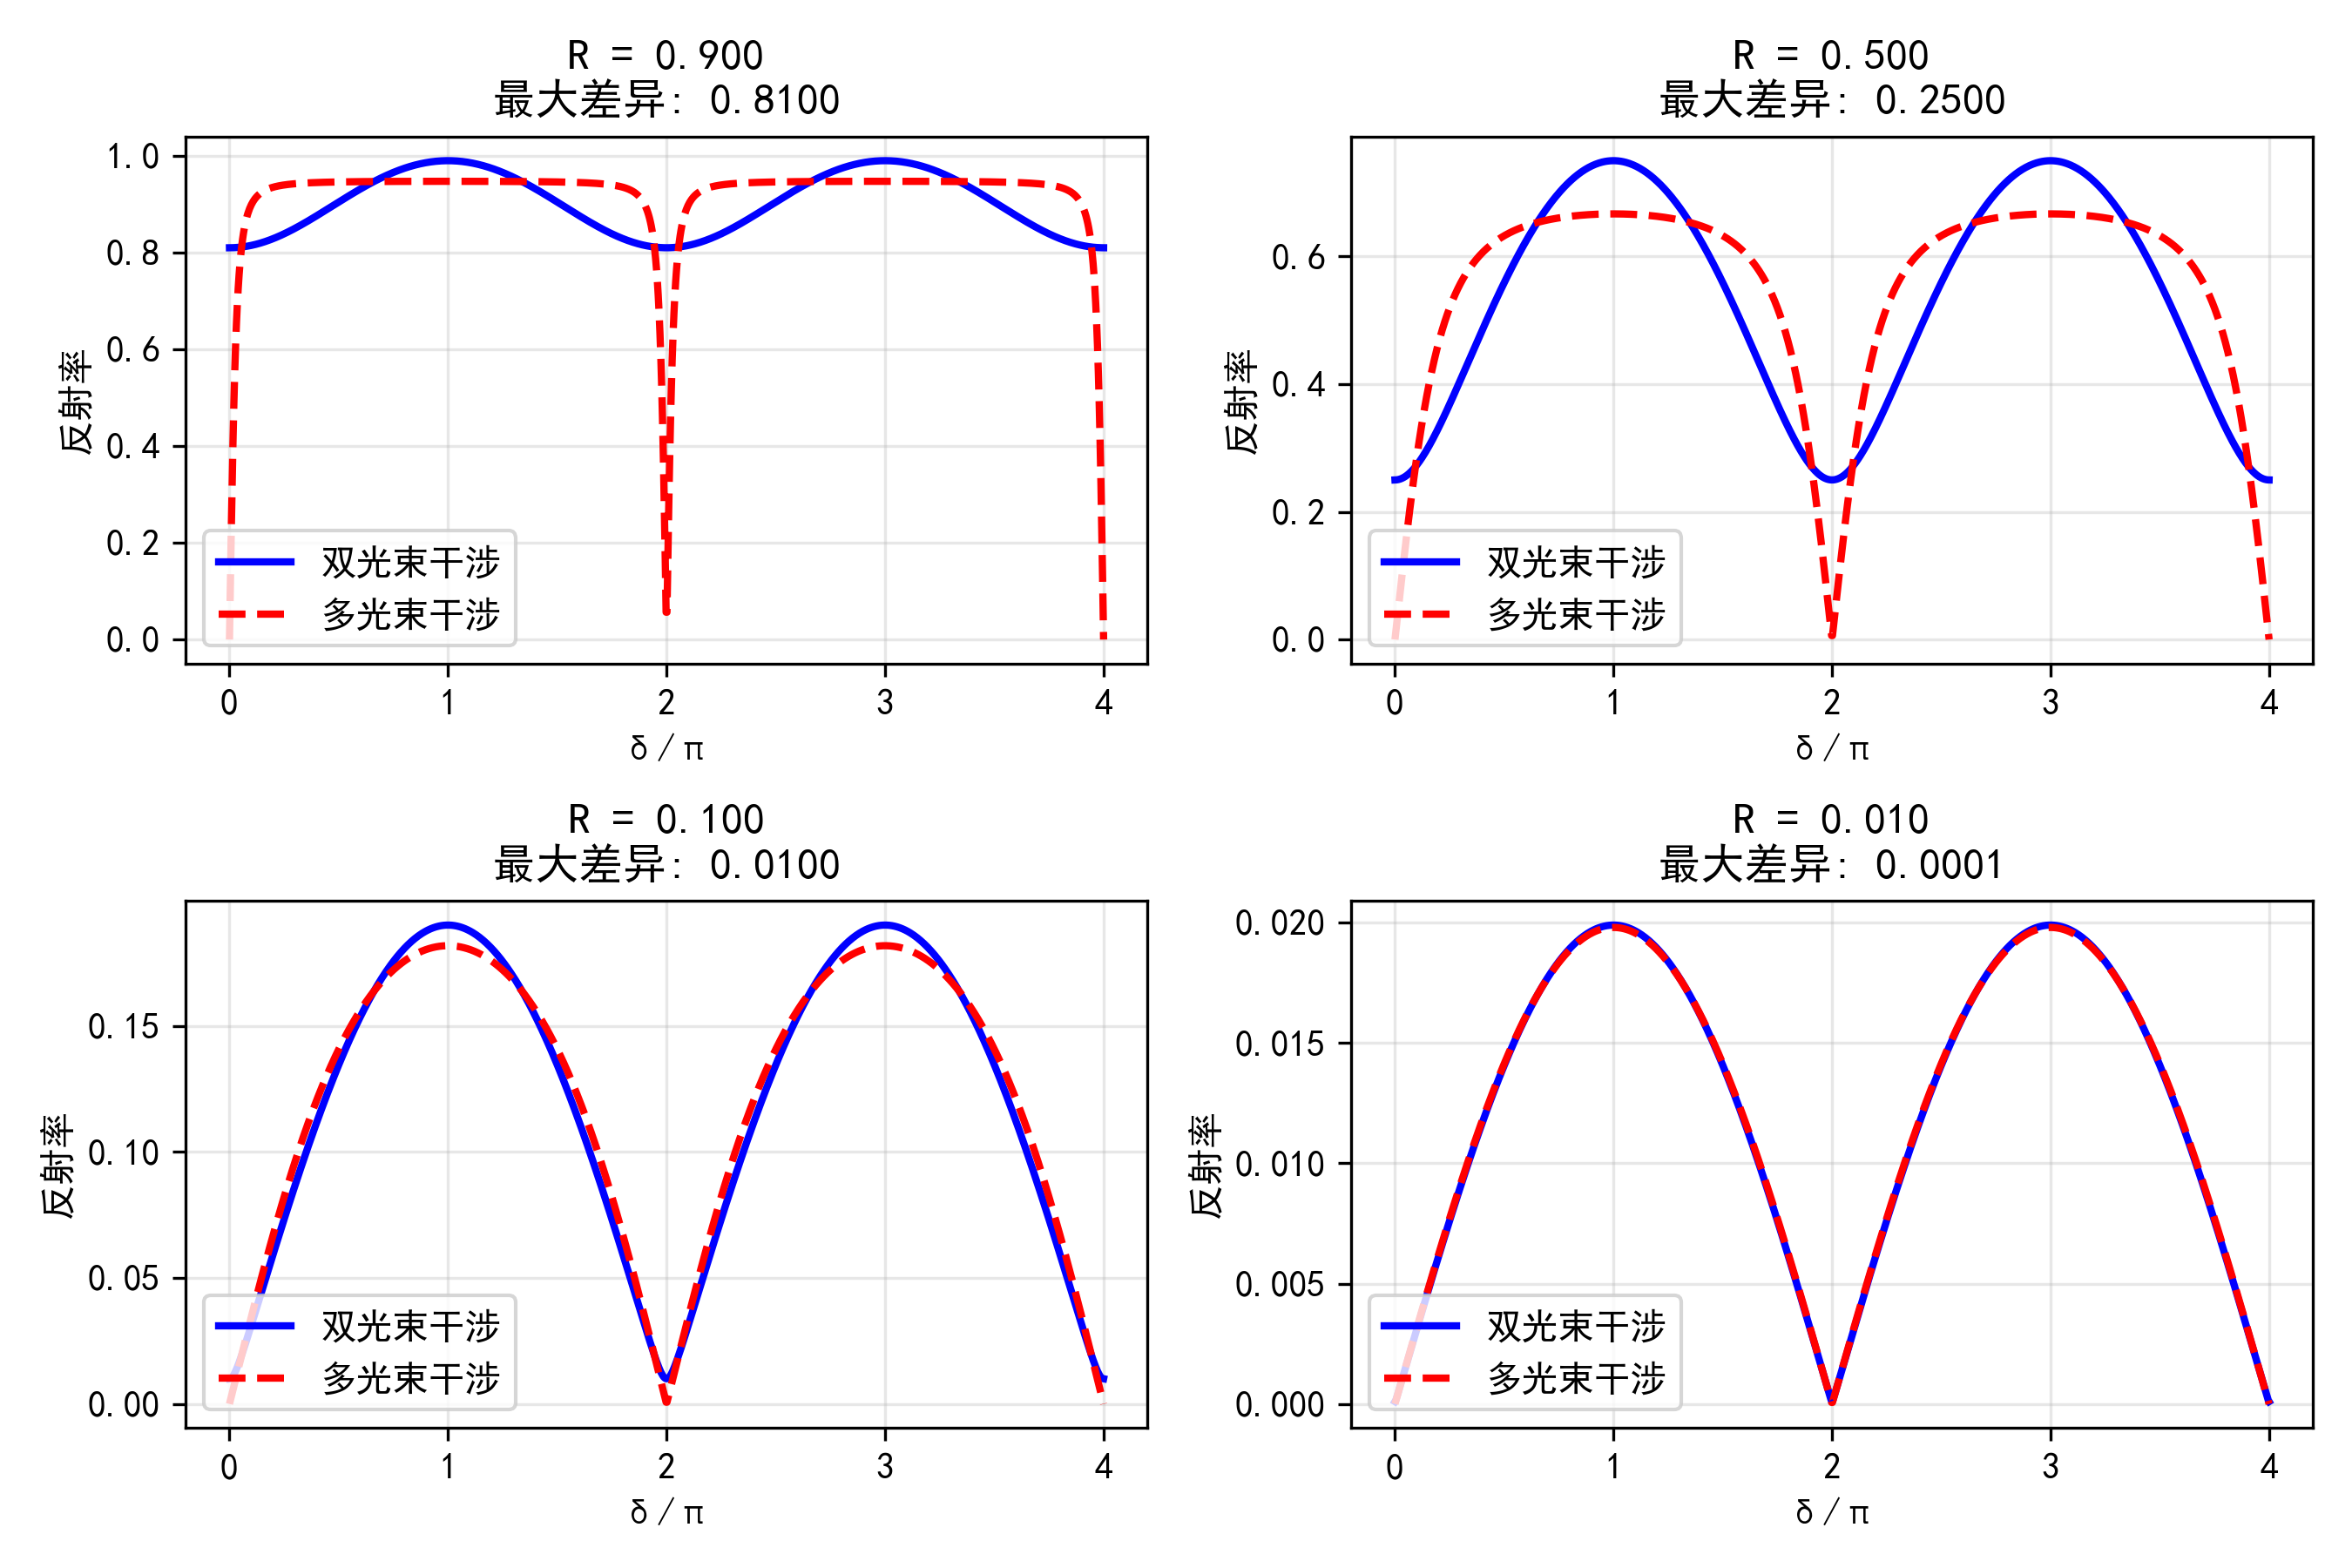
\includegraphics[height=0.35\textheight]{p5.png}
	\end{minipage}  
	\caption{反射率函数示意图}
\end{figure}\par 
降低多光束干涉后附件1和附件2求解得到的外延层厚度分别为16.2416$\mu m$和17.4144$\mu m$，整体影响不大。\par 
\section{模型评价}
\subsection{模型的优点}
1.理论依据扎实，融合光学干涉与材料色散模型，构建了完整的外延层厚度计算体系。\par

2.双光束与多光束干涉模型分别建立，适应不同实测场景，模型适用性与推广性强。
\par
3.通过波谷分析和滤波降噪处理数据，有效提升信噪比，厚度计算结果稳定可靠。\par
\subsection{模型的缺点}
1.模型假设较多，如衬底无吸收、环境折射率为1，在实际复杂环境中易引入误差。\par

2.折射率计算依赖载流子浓度等经验参数，缺乏实测校准，影响模型泛化能力。\par
%Reference
\begin{thebibliography}{40}
	\bibitem{1}赵凯华,钟锡华 编.光学[M].北京：北京大学出版社,2018
	\bibitem{2}张继涛,黄沛,李岩,等.标准状态下氮气在0.145～2.058μm的色散特性[J].光学学报,2012
	\bibitem{3}全国半导体设备和材料标准化技术委员会(SAC/TC 203),全国半导体设备和材料标准化技术委员会材料分技术委员会(SAC/TC 203/SC 2).碳化硅外延层厚度的测试　红外反射法:GB/T 42905-2023[S].中国标准出版社,2023
	
	\bibitem{4}K. D. Möller.Optics[M].纽约:施普林格出版社,2007
	\bibitem{5}豆包，Version：10.2.0，字节跳动，2025-09-06
	\bibitem{6}Deepseek ,DeepSeek-V3.1,深度求索(DeepSeek),2025-09-06
	\bibitem{7}梁铨廷.物理光学（第4版）.北京：电子工业出版社,2012
	\bibitem{8}Jiaxing Sun, Xinyu Li, Haojie Zhang, Jinlong Song, Zhisong Li,
	A method for measuring and calibrating the thickness of thin films based on infrared interference technology,
	Results in Physics,
	Volume 51,
	2023
	\bibitem{9}李志云.基于FTIR技术的4H-SiC同质外延材料的测试[D].西安电子科技大学,2010.
	\bibitem{10}MF. MACMILLAN, A. HENRY, and E. JANZEN.“Thickness Determination ofLow Doped SiC Epi-Films on Highly Doped SiC Substrates”. Journal of ElectronicMaterials.1998.
\end{thebibliography}
\newpage
\newgeometry{left=1.50cm,right=0.5cm,top=3.00cm,bottom=3.0cm}	%修改附录代码的几何页面
\begin{center}
	\sihao \heiti 附录
	
	\fontsize{10pt}{16pt}		\selectfont	
	\begin{lstlisting}[ language=python,numbers=left,numberstyle=\tiny,keywordstyle=\color{blue!70},commentstyle=\color{red!50!green!50!blue!50},frame=shadowbox, rulesepcolor=\color{red!20!green!20!blue!20},escapeinside=``,xleftmargin=2em,xrightmargin=2em,aboveskip=1em] 
		%%%折射率计算：
		def calculate_refractive_index(wavenumber):
		refractive_index = (6.52 * (1 + (970.1**2 - 793.9**2) / (793.9**2 - wavenumber**2) - 1.6 * 10**5 /
		(wavenumber**2 * 4 * 3.1415926 * 3.1415926 *10^(20)*9* 9 * 10**16 * 0.42 * 6.52 * 8.85 * 10**(-12))))
		refractive_index = refractive_index.apply(lambda x: 0 if isinstance(x, complex) else x)
		refractive_index = refractive_index.apply(lambda x: x**0.5 if x >= 0 else 0)
		return refractive_index
		
		%%%统计可能的波峰并计算相关统计参数：
		def detect_valleys_and_analyze_differences(wavenumber, reflectance):
		if len(reflectance) > 51:
		smoothed_reflectance = savgol_filter(reflectance, 51, 3)
		else:
		smoothed_reflectance = reflectance
		
		mean_reflectance = reflectance.mean()
		std_reflectance = reflectance.std()
		height_threshold = -(mean_reflectance - 0.3 * std_reflectance)
		valleys_idx, properties = find_peaks(-smoothed_reflectance, 
		height=-50,
		distance=10,
		prominence=std_reflectance * 0.05)
		if len(valleys_idx) == 0:
		print("未检测到明显的波谷")
		return None
		
		valley_wavenumbers = wavenumber.iloc[valleys_idx]
		valley_reflectances = reflectance.iloc[valleys_idx]
		print(f"检测到 {len(valleys_idx)} 个波谷：")
		
		valley_info = []
		for i, (idx, wn, refl) in enumerate(zip(valleys_idx, valley_wavenumbers, valley_reflectances)):
		valley_info.append({
			'波谷编号': i + 1,
			'数据点索引': idx,
			'波数 (cm⁻¹)': wn,
			'反射率': refl
		})
		print(f"  波谷 {i+1}: 波数 {wn:.2f} cm⁻¹, 反射率 {refl:.6f}")
		
		if len(valleys_idx) > 1:
		wavenumber_differences = []
		reflectance_differences = []
		interval_info = []
		
		for i in range(len(valleys_idx) - 1):
		wn_diff = valley_wavenumbers.iloc[i+1] - valley_wavenumbers.iloc[i]
		refl_diff = valley_reflectances.iloc[i+1] - valley_reflectances.iloc[i]
		
		wavenumber_differences.append(wn_diff)
		reflectance_differences.append(refl_diff)
		interval_info.append({
			'区间': f'波谷{i+1} → 波谷{i+2}',
			'波数差值 (cm⁻¹)': wn_diff,
			'反射率差值': refl_diff,
			'起始波数': valley_wavenumbers.iloc[i],
			'结束波数': valley_wavenumbers.iloc[i+1]
		})
		print(f"  波谷{i+1} → 波谷{i+2}: 波数差值 {wn_diff:.2f} cm⁻¹, 反射率差值 {refl_diff:.6f}")
		
		wn_diff_array = np.array(wavenumber_differences)
		refl_diff_array = np.array(reflectance_differences)
		print(f"波数差值统计:")
		print(f"  平均差值: {wn_diff_array.mean():.2f} cm⁻¹")
		print(f"  标准差: {wn_diff_array.std():.2f} cm⁻¹")
		print(f"  最小差值: {wn_diff_array.min():.2f} cm⁻¹")
		print(f"  最大差值: {wn_diff_array.max():.2f} cm⁻¹")
		print(f"  差值范围: {wn_diff_array.max() - wn_diff_array.min():.2f} cm⁻¹")
		print(f"\n反射率差值统计:")
		print(f"  平均差值: {refl_diff_array.mean():.6f}")
		print(f"  标准差: {refl_diff_array.std():.6f}")
		print(f"  最小差值: {refl_diff_array.min():.6f}")
		print(f"  最大差值: {refl_diff_array.max():.6f}")
		wn_diff_cv = wn_diff_array.std() / wn_diff_array.mean() if wn_diff_array.mean() != 0 else 0
		
		return {
			'valleys_idx': valleys_idx,
			'valley_wavenumbers': valley_wavenumbers,
			'valley_reflectances': valley_reflectances,
			'valley_info': valley_info,
			'interval_info': interval_info,
			'wavenumber_differences': wavenumber_differences,
			'reflectance_differences': reflectance_differences,
			'wn_diff_stats': {
				'mean': wn_diff_array.mean(),
				'std': wn_diff_array.std(),
				'min': wn_diff_array.min(),
				'max': wn_diff_array.max(),
				'cv': wn_diff_cv
			},
			'refl_diff_stats': {
				'mean': refl_diff_array.mean(),
				'std': refl_diff_array.std(),
				'min': refl_diff_array.min(),
				'max': refl_diff_array.max()
			}
		}
		else:
		return {
			'valleys_idx': valleys_idx,
			'valley_wavenumbers': valley_wavenumbers,
			'valley_reflectances': valley_reflectances,
			'valley_info': valley_info
		}
		
		%%%计算理论反射率：
		def theoretical_reflectance(D, wavelength, n, R_measured, theta_deg=10):
		theta = np.deg2rad(theta_deg)
		delta = (4 * np.pi / wavelength) * n * D * np.cos(theta)
		r=np.sqrt(0.5*(((np.cos(theta)-np.sqrt(n**2-np.sin(theta)**2))/(np.cos(theta)+np.sqrt(n**2-np.sin(theta)**2)))**2+((n*np.cos(theta)-np.sqrt(n**2-np.sin(theta)**2)/n)/(n*np.cos(theta)+np.sqrt(n**2-np.sin(theta)**2)/n))**2))
		r_prime = r  
		exp_i_delta = np.exp(1j * delta)
		numerator = r + r_prime * exp_i_delta
		denominator = 1 - R_measured * exp_i_delta
		R_theory = np.abs(numerator / denominator) ** 2
		
		return R_theory
		
		%%%用最小二乘法拟合厚度：
		def solve_thickness_lm(wavelength, n, R_measured, D_initial=4, D_bounds=(0.1, 50)):
		result = least_squares(
		residual_function,
		x0=[D_initial],
		args=(wavelength, n, R_measured),
		method='trf',  # Trust Region Reflective algorithm
		bounds=(3, 10),
		loss='linear',
		ftol=1e-8,
		xtol=1e-8,
		gtol=1e-8,
		max_nfev=1000
		)
		
		return result
		
	\end{lstlisting}
\end{center}
\end{document}